\chapter{\uppercase{Impact of Geometry of Output Quantities on Consistent Solutions} \label{chapter:geometry}}

Here, we motivate the reduction of a quantity called \emph{skewness} in pursuit of optimizing the geometry of solutions to SIPs with respect to their ability to be well-approximated with random sampling.
However, the results hold for any attempt to approximate densities defined on sets induced by random samples, and thus may be of interest to the larger research community.

We demonstrate that the number of samples required to approximate densities using uniform i.i.d.~sampling is proportional to the skewness of the map used for inversion, though the convergence rate of the algorithm used to solve the SIP is unaffected.
We focus on the accuracy of the consistent solutions to the SIP.
It is illustrative to begin with the original set-based approximations to solutions developed in \cite{BGE+15, BET+14, MBD+15} as the dependence of solutions on skewness is more explicit than in the density-based approach.

%%%%%

\section{Set-Based Inversion for Consistent Measures}\label{sec:set-based}
% Intro
To properly summarize the set-based solution, we define several measure/probability spaces and refer to the schematic given in Figure \ref{fig:scheme} in order to illustrate the steps and spaces required in the formulation and solution of the SIP.
For a more extensive review, we refer the reader to \cite{BBE11}, \cite{BES12}, and \cite{BET+14}.
Additional background and extensions of this theory are available in the PhD theses of Lindley Graham (UT Austin), Scott Walsh (UCD), Lei Yang (CSU) [TK - cite 3].

%%%%%%%%%%%%%%%%%%%%%%%%
\begin{figure}[!h]
\begin{equation}
\underbrace{
\underbrace{
\overbrace{
 \Pspace \xmapsto{\  \qoi \ } \Dspace
  \xmapsto{\ \observedP \ } \Ospace
 }^{
 \text{(S1): Stochastic Inverse Problem (SIP)}
 }
 \xmapsto{\ \qoi^{-1} \ } (\pspace, \cborel, \contourP)
 }_{
 \text{(S2): Solution to SIP Satisfying Eq. \eqref{eq:dataspace_pushforward_measure}}}
 \xmapsto{\ \set{\PP_\ell}_{\ell\in\mathcal{L}} \ } (\pspace, \pborel, \paramP)
 }
 _{
 \text{(S3): Unique Solution to SIP by Eq.~\eqref{eq:disintegration_measure} and Ansatz}
 }
\end{equation}
\caption{The first step (S1) defines (i)~the formulation of the SIP by specification of the model, (ii)~the measure spaces of parameters and (iii)~observable outputs, and (iv)~the probability measure on the latter. The second step (S2) defines a unique solution to the SIP on the space $\pspace$ equipped with the contour $\sa$ $\cborel$ using the definition of the push-forward measure. In (S3), the Disintegration Theorem and and Ansatz are applied to define a unique solution on the space of interest $(\pspace, \pborel)$ equipped with a probability measure $\paramP$.}
\label{fig:scheme}
\end{figure}


The initial measure/probability spaces involved in the formulation of the SIP are summarized in step (S1) of Fig.~\ref{fig:scheme}, starting with measure space $\Pspace$.

The assumption that $\qoi$ is at least piecewise-differentiable implies the measurability of the QoI map, so that the space $\dspace$ induced by $\qoi$ is equipped with the Borel $\sa$ $\dborel$ \cite{Hunter}.
The ``push-forward'' measure $\dmeas$ on ${(\dspace, \dborel)}$ is defined as

\begin{equation}\label{eq:dataspace_pushforward_measure}
\dmeas (A) = \int_A \, d\dmeas := \int_{\qoi^{-1}(A)} \, d\pmeas = \pmeas \left (\qoi^{-1}(A) \right ) \quad \forall \;  A\in\dborel,
\end{equation}

\noindent which defines the measure space $\Dspace$\footnote{When referring to properties of the data space that are not unique to the choice of map used to induce $\dspace$, we will drop the subscript notation and assume the dependence is understood, as expressed in Fig.~\ref{fig:scheme}.}.

In practice, when $\dmeas$ is absolutely continuous with respect to the $\dimD$--dimensional Lebesgue measure, we substitute the Lebesgue measure for $\dmeas$.

The final step in (S1) involves the specification of a probability measure $\dataP$ (absolutely continuous with respect to $\dmeas$) on ${(\dspace, \dborel)}$ to model the uncertainty in data.
This leads to the SIP from Def.~\eqref{defn:inverse-problem}: determine a probability measure $\paramP$ on ${(\pspace, \pborel)}$ such that

\begin{equation}\label{eq:inverse_measure}
\paramP \left ( \qoi^{-1}(E)\right ) = \dataP(E) \; \forall \; E \in \dborel.
\end{equation}

This equation implies that any solution is uniquely determined on the induced contour $\sa$
\begin{equation}\label{eq:contour_sa}
\cborel = \set{\qoi^{-1}(E) : E \in \dborel } \subset \pborel,
\end{equation}
which is summarized as step (S2) of Fig.~\ref{fig:scheme}.
However, for sets $A \in \pborel \setminus \cborel$, more information is required than is provided in Eq.~\eqref{eq:inverse_measure} in order to determine $\paramP (A)$.
When solutions to the SIP are given by densities, we form a family of conditional densities using an initial density.
In the set-based approach, we do not assume an initial density on $(\pspace, \pborel)$.
Instead, we consider approximations of contour events.
Below, we describe these structures and the relationship to the Disintegration theorem.

By the Implicit Function Theorem, if $\qlam \in C^1 (\pspace)$ and we let $\data\in\dspace$ be a fixed datum, $\qoi^{-1}(q)$ exists as a $(\nparams-\ndata)$\--dimensional manifold (possibly piecewise-defined) that we refer to as a \emph{generalized contour} \cite{BET+14}.
These generalized contours can be indexed by a $\dimD$--dimensional manifold (also possibly piecewise-defined) of dimension $\ndata$ called a \emph{transverse parameterization} that intersects each contour once and only once.
In \cite{BET+14}, it is shown that transverse parameterizations are guaranteed to exist and can be approximated by a finite number of $\dimD$---dimensional hyperplanes when $\pspace$ is compact.
In general, the transverse parameterization is not unique.

We let $\LL$ denote any particular transverse parameterization.
Each $\ell\in\LL$ corresponds to a unique generalized contour $\CC_\ell \in \pspace$ and each point $\param\in\pspace$ belongs to a unique $\CC_\ell\in\pspace$.
Thus, a transverse parameterization defines a bijection between the manifold $\LL$ and the partitioning of $\pspace$ into generalized contours that decomposes $\pspace$ in terms of equivalence classes.
The induced $\sa$ $\cborel$ and this bijection can then be used to define the measurable space $(\LL, \BB_\LL)$.

We denote the projection map $P_\LL : \pspace \to \LL$, and let $\set{\CC_\ell}_{\ell\in\LL}$ represent the family of generalized contours indexed by $\LL$, yielding the associated family of measurable spaces $\set{\left ( \CC_\ell, \BB_{\CC_\ell} \right )}_{\ell\in\LL}{}$.
By the Disintegration Theorem [TK - cite], any $\paramP$ is now defined completely in terms of structures embedded in $(\pspace, \pborel)$ as a (marginal) probability measure $\PP_\LL$ on $(\LL, \BB_\LL)$ and a family of (conditional) probability measures $\set{\PP_\ell}_{\ell\in\LL}$ on $\set{\left ( \CC_\ell, \BB_{\CC_\ell} \right )}_{\ell\in\LL}$ such that
\begin{equation}\label{eq:disintegration_measure}
\paramP (A) = \int_{P_\LL(A)} \left ( \int_{P_{\LL}^{-1} (\ell) \cap A}\, d\PP_\ell(\param) \right )\, d\PP_\LL (\ell), \; \forall \; A \in \pborel
\end{equation}

The disintegration of Eq.~\eqref{eq:disintegration_measure} implies that a specification of a family of conditional probability measures $\set{P_\ell}_{\ell\in\LL}$ gives us a unique solution to the SIP on ${(\pspace, \pborel)}$ since the marginal $\PP_\LL$ on ${(\LL, \BB_\LL)}$ is uniquely determined by $\observedP$ on ${(\dspace, \dborel)}$.

The conditional measures are not determined by the specification of $\dataP$.
We follow the work of \cite{BET+14} and adopt the \emph{standard ansatz} determined by the disintegration of the measure $\pmeas$ to compute probabilities of sets contained within contour events whenever $\pmeas(\pspace) < \infty$, e.g. when $\pmeas$ is the $\dimP$--dimensional Lebesgue measure and $\pspace \in \RP$ is precompact.
The standard ansatz is given by

\begin{equation}\label{eq:standard_ansatz}
\PP_\ell = \mu_{\CC_\ell} / \mu_{\CC_\ell}(\CC_\ell), \; \forall \; \ell \in \LL,
\end{equation}

\noindent where $\mu_{\CC_\ell}$ is the disintegrated volume measure on generalized contour $\CC_\ell$.
Thus, we have defined a unique solution to the SIP on ${(\pspace, \pborel)}$, completing step (S3) in Fig.~\ref{fig:scheme}.

In the absence of other information about differences in relative likelihoods of parameters, the standard ansatz effectively implies a uniform distribution describing the initial state of uncertainty about the input parameters\footnote{In the event that $\pspace$ is compact.}.
In the vocabulary of the density-based approach, the measure $\paramP$ can be viewed as updating an initial uniform measure on $\pspace$ in directions informed by the Quantity of Interest map, given uncertain data characterized by $\dataP$.
However, unlike the density-based approach that utilizes the pushforward of an initial density in the construction of a solution, the ansatz is imposed only on contours in $\pspace$.
Moreover, this does not assume any absolute continuity of probability measures.

\vfill

%% \subsubsection{Alternative Derivation Using Bayes' Rule}\label{sec:set_bayes}
In the measure-theoretic approach studied in~\cite{BBE11, BET+14}, Voronoi-cell discretizations of $\pspace$ are used to construct set-valued approximations of the updated measure directly, so we refer to it as the \emph{explicit} approach.
By contrast, sampling from densities is an \emph{implicit} approach, and is discussed in greater detail in \ref{sec:ch02-sample}.
Here, we provide a ``set-based'' derivation of the updated measure to more easily compare to the explicit approximation of the solution given measure in~\cite{BET+14}.

First, we start by observing that if $A, B \subset \pspace$ such that $A = \qoi^{-1}(\qoi(B))$, then we have that $B\subset A$ (the inclusion may be proper).
Therefore, for any probability measure $P$ on $(\pspace, \pborel)$, 
\[
P(B) = P(B|A) \, P(A).
\]
If $P$ is intended to solve the inverse problem, then we are motivated to take
\[
P(A) = \observed (\qoi(A)) = \observed (B),
\]
in the above formula.

We must now determine how to properly define $P(B|A)$. 
We leverage Bayes' Theorem~\cite{Smith} in order to utilize the prior density on contour events.
In other words, we use the prior $\initialP$ on $(\pspace, \pborel)$ and Bayes' Theorem to get
\begin{equation}\label{eq:bayes_full}
P(B|A) = \initialP(B|A) = \frac{ \initialP(A|B) \initialP(B) }{ \initialP(A) },
\end{equation}
and since $B \subset A$, $\initialP(A|B) = 1$, \eqref{eq:bayes_full} simplifies to

\begin{equation}\label{eq:bayes}
\initialP(B|A) = \frac{ \initialP(B) }{ \initialP(A) }.
\end{equation}

Recall from \eqref{eq:predicted} that $\predictedP$ is the push-forward of the prior, giving $\initialP(A) = \predictedP (\qoi(A)) = \predictedP \left (\qoi(B)\right )$, which then gives the following set-valued ``solution'' to the stochastic inverse problem:
\begin{equation}\label{eq:sip_sol_cont}
\updatedP(B) := \begin{cases}
\initialP(B) \frac{ \observed(B) }{ \predictedP \left (\qoi(B)\right ) ) } & \text{ if } \initialP(B) > 0,\\
0 & \text{ otherwise}.
\end{cases}
\end{equation}

This set-valued update is only a solution on certain (sub-)$\sigma$-algebras of $\pborel$. 
Nonetheless, we can form explicit approximations to the update, e.g. as done in~\cite{BET+14, BES12, BBE11}. 
In other words, an Ansatz is used in place of the prior; it serves the same purpose to distribute probabilities in directions not informed by the QoI map.

However, such an explicit approach requires an approximation of \emph{events in $\pborel$}. 
This is in direct contrast to the numerical approximation of the density $\updated$ that only requires approximation of $\predicted$.
Since we often expect the dimension of $\dspace$ to be less than the dimension of $\pspace$, this can prove to be a significant numerical advantage for the ``implicit'' approximation given by the updated probability density function. 

% Numerical Approximation
\subsection{Numerical Approximation and Analysis}\label{sec:set-algorithm}
We present a non-intrusive algorithm based on Monte Carlo sampling\---initially introduced in \cite{BET+14} and further analyzed in \cite{BET+14-arxiv}\---that is structured in four stages (written as four independent for-loops), that are linked to the stages in Fig.~\ref{fig:scheme}.
We direct the interested reader to \cite{BET+14-arxiv} for more detailed information and analysis of this algorithm, e.g., on the requirement of a sampler being ``$\pborel$-consistent'' to ensure convergence.


\begin{algorithm}[hbtp]
\DontPrintSemicolon
Choose a discretization partition $\set{D_\idisc}_{\idisc=1}^{\ndiscs}$ of $\dspace$.\\
	\For{$\idisc = 1, \hdots, \ndiscs$}{
			Compute $p_{\dspace, \idisc} = \dataP(D_\idisc)$.
	}
 	Choose samples $\set{\param^{(\iparam)}}_{\iparam=1}^{\nsamps} \subset \pspace$, which implicitly defines a Voronoi-cell partition $\set{\VV_\iparam}_{\iparam=1}^{\nsamps}$ of $\pspace$.\\
	\For{$\iparam = 1, \hdots, \nsamps$}{
	Compute $\qoi_\iparam = \qoi(\param^{(\iparam)})$.\\
	Let $\OO_\idisc = \set{\iparam: \qoi_\iparam \in D_\idisc}$.\\
	Compute approximations $V_\iparam \approx \pmeas (\VV_\iparam)$.
	}
	\For{$\idisc = 1, \hdots, \ndiscs$}{
	Compute $\CC_\idisc = \set{\iparam:Q_\iparam \in D_\idisc}$.
	}
	\For{$\iparam = 1, \hdots, \nsamps$}{
	Compute $p_{\pspace, \iparam} = \left ( V_\iparam / \sum_{j\in \CC_{\OO_\iparam} } V_j \right ) p_{\dspace, \OO_\iparam}$.
	}
	For any $A\in \pborel$, compute
	\begin{equation}
	\PP_{\pspace, \ndiscs, \nsamps} (A) = \sum_{\iparam=1}^\nsamps p_{\pspace, \iparam} \Chi_{\VV_\iparam} (A)
	\end{equation}
 \caption{Numerical Approximation of the Inverse Density}
 \label{alg:inv_density}
\end{algorithm}


The first two stages correspond to formulating the discretized version of the SIP given in step (S1) in Fig.~\ref{fig:scheme}.
We first discretize the probability space $\Ospace$.
Then, we simultaneously discretize the measure space $(\pspace, \pborel, \pmeas)$ and construct a simple-function approximation to the map $\qoi$.
These stages introduce the primary sources of error, and the third and fourth stages may be thought of as solving the discretized SIP exactly.
The samples that are used to describe $\pspace$ implicitly define a set of Voronoi cells $\set{\VV_\iparam}_{\iparam=1}^{\nsamps}$, which can be seen in Figure~\ref{fig:voronoi_cells}.
Each sample set defines a fundamentally different geometry.

\begin{figure}[ht]
\centering
	\begin{minipage}{.475\textwidth}
		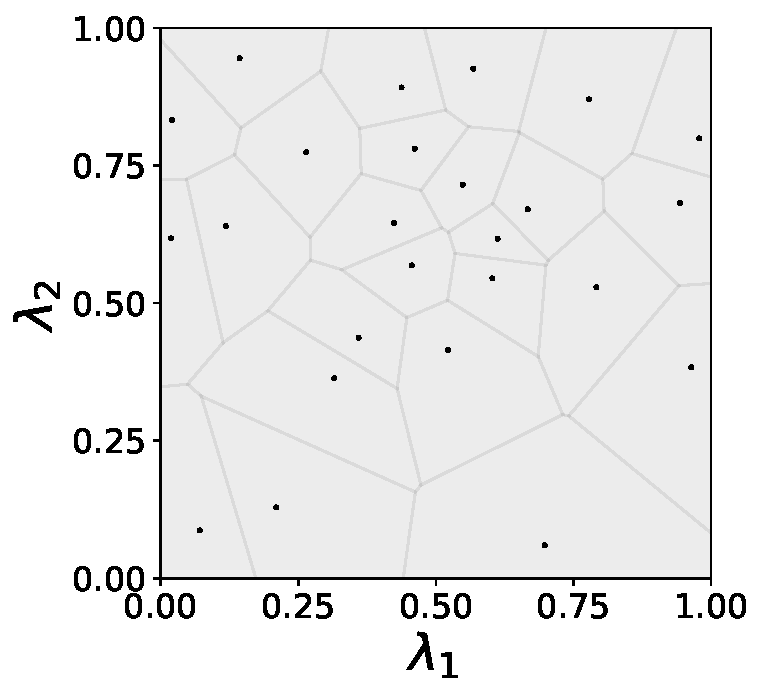
\includegraphics[width=\linewidth]{./images/voronoi_diagrams/voronoi_diagram_N25_r0}
	\end{minipage}
\caption{
Voronoi-cell discretization (partition) induced by $\nsamps = 25 $ uniform i.i.d.~random samples in $\pspace = [0,1]^2$.
}
\label{fig:voronoi_cells}
\end{figure}

The third stage then identifies the collection of Voronoi cells in $\pspace$ that approximate the contour events in $\cborel$ defined by $\qoi^{-1}(D_\idisc)$ for $\idisc=1,\hdots,\ndiscs$. This allows us to formulate the consistent solution to the discretized SIP on $(\pspace, \cborel, \contourP)$ as illustrated in step (S2) of Fig.~\ref{fig:scheme}.
The fourth stage, associated with step (S3) in Fig.~\ref{fig:scheme}, uses a discrete version of the ansatz to approximate the probability of $\VV_\iparam$ for $\iparam=1,\dots,\nsamps$.
This results in an approximate probability measure, denoted by $\updatedPxNM$, which produces the same probability estimates for events $A$ and $A\setminus \set{ \param^{(\iparam)} }_{\iparam=1}^\nsamps$, which are identical almost everywhere with respect to $\pmeas$.

Note that Algorithm~\ref{alg:inv_density} makes no mention of the method by which the samples $\set{ \param^{(\iparam)} }_{\iparam=1}^{\nsamps}$ were generated or sets in $\set{D_\idisc}_{\idisc=1}^{\ndiscs}$ are chosen.
$\set{ \param^{(\iparam)} }_{\iparam=1}^{\nsamps}$ may be generated using uniform random sampling, Latin-hypercube sampling, or even regular grids.
A thorough discussion of the choices involved in making such decisions is beyond the scope of this work, though we touch briefly on the discretization of $\dspace$ in the following section.


% Descriptions of Error
\subsection{Descriptions of Error}\label{sec:set-error}

Recall that we assumed $\dataP$ is absolutely continuous with respect to $\dmeas$, which allows us to describe $\dataP$ with a density $\rho_\dspace$. Then, for any partition $\set{D_\idisc}_{\idisc=1}^{\ndiscs}$ of $\dspace$,
\[
\dataP (D_\idisc) = \int_{D_\idisc} \observed \, \dmeas, \quad \text{ for } \idisc = 1, \hdots, \ndiscs.
\]

We often use Monte Carlo approximations to compute the approximations $p_{\dspace, \idisc}=\dataP(D_\idisc)$ in the first for-loop in Algorithm~\ref{alg:inv_density}.
These samples are generated on $\dspace$ and do not require numerical solutions to the model.
We therefore assume that for any discretization of $\dspace$, these approximations can be made sufficiently accurate and neglect the error in this computation.

We denote the exact solution to the SIP associated with this partitioning of $\dspace$ by $\PP_{\pspace, \ndiscs}$.
In situations where $\qoi(\param^{(\iparam)})$ is estimated (e.g. by application of a functional on a finite-element solution to a PDE), the approximate solutions to the SIP given in the final for-loop of Algorithm~\ref{alg:inv_density} are denoted by $\PP_{\pspace, \ndiscs, \nsamps, h}$.
Here, the $h$ is in reference to a mesh or other numerical parameter that determines the accuracy of the numerical solution $u_h(\param^{(\iparam)})\approx u(\param^{(\iparam)})$, and subsequently the accuracy in the computations of $\qoi_\iparam = \qoi(\param^{(\iparam)})$ in Algorithm~\ref{alg:inv_density}.
Then, by repeated application of the triangle inequality,
\begin{equation}
\label{eq:set-triangleineq}
d(\PP_{\pspace, \ndiscs, \nsamps, h}, \paramP) \leq
\underset{ \text{(E1)} }{\underbrace{d(\PP_{\pspace, \ndiscs, \nsamps, h},\PP_{\pspace, \ndiscs, \nsamps})}} +
\underset{ \text{(E2)} }{\underbrace{d(\PP_{\pspace, \ndiscs, \nsamps}, \PP_{\pspace, \ndiscs}) }}+
\underset{ \text{(E3)} }{\underbrace{d(\PP_{\pspace, \ndiscs}, \paramP) }}.
\end{equation}

The term (E1) describes the effect of the error in the numerically evaluated $\qoi_\iparam$ on the solution to the SIP.
The term (E2) describes the effect of finite sampling error in $\pspace$ on the solution to the SIP and (E3) describes the effect of discretization error of $\dataP$ on the solution to the SIP.

We assume that $h$ is tunable so that for any $A\in \pborel$,
\[
\lim\limits_{h \downarrow 0} \PP_{\pspace, \ndiscs, \nsamps, \imesh} (A) = \PP_{\pspace, \ndiscs, \nsamps} (A).
\]
It is possible to prove the convergence of $\PP_{\pspace, \ndiscs, \nsamps, \imesh} (A) \to \paramP (A)$ for some $A\in \pborel$ and on estimating the error in $\PP_{\pspace, \ndiscs, \nsamps, h}(A)$.
For example, in \cite{BGE+15}, adjoint-based a posteriori estimates in the computed QoI are combined with a statistical analysis to both estimate and bound the error in $\PP_{\pspace, \ndiscs, \nsamps, \imesh} (A)$.
In [TK - cite JNME 2019], adjoints are used to compute both error and derivative estimates of $\qoi(\param^{(\iparam)})$ to improve the accuracy in $\PP_{\pspace, \ndiscs, \nsamps, \imesh} (A)$.
Since the error due to $\imesh$ can be estimated as described in previous studies, and $\ndiscs$ can be made arbitrarily large, we neglect (E1) and (E3) here.
Thus, we limit our focus to (E2), where certain geometric properties of the QoI map are known to significantly impact this term, as we show below.



\section{Skewness and Information Content}\label{sec:skewness}
In \cite{BGE+15}, the concept of skewness in a QoI map $\qoi$ is introduced, quantified, and related to the accuracy in solving the stochastic inverse problem with a finite number of samples.
In effect, skewness is a geometric property that describes how the right angles in generalized rectangles belonging to $\dborel$ are transformed by $\qoi^{-1}$.
An a priori analysis demonstrated that the number of samples from a {\em regular uniform grid} in $\pspace$ required to approximate the $\pmeas$-measure of $\qoi^{-1}(E)$ to a desired level of accuracy is proportional to the skewness of $\qoi$ raised to the ($d-1$) power where $d$ is the dimension of $\dspace$.
This is a version of the so-called curse-of-dimension for the set-based approach.

Skewness is explored further in \cite{Walsh} in the context of optimal experimental design.
There, an additional geometric property of $\qoi$ related to the \emph{precision} in the solution of the associated stochastic inverse problem is introduced and quantified.
For completeness, we define skewness below and refer the interested reader to \cite{BGE+15, BPW17, Walsh} for more details.

\begin{defn}
For any QoI map $\qoi$, $\param \in \pspace$, and a specified row vector $\bf{j}_k$ of the Jacobian $J_{\param, Q}$, we define
\begin{equation}
S_\qoi(J_{\param,Q}, \bf{j}_k) := \frac{\abs{\bf{j}_k} }{\abs{\bf{j}_k^\perp}}.
\label{eq:skewness}
\end{equation}

We define the \textbf{local skewness} of a map $\qoi$ at a point $\pspace$ as
\begin{equation}
S_\qoi(\param) := \max_{1\leq k \leq d} S_\qoi(J_{\param,Q}, \bf{j}_k).
\label{eq:localskewness}
\end{equation}
\end{defn}

\begin{defn}
The \textbf{average} \emph{(or \textbf{expected})} \textbf{skewness} is defined as
\begin{equation}
\overline{S_Q} := \frac{1}{\mu_{\pspace}(\pspace)} \int_\pspace S_Q (\param) \, d\mu_{\pspace}
\label{eq:avgskew}
\end{equation}
\end{defn}

In \cite{BPW17}, it is shown that $S_\qoi(\param)$ is efficiently computed using a singular value decomposition (SVD) of the Jacobian $J_{\param,\qoi}$, i.e., we randomly sample $J_{\param,\qoi}$ and compute the SVDs.
In general, we approximate $\overline{S_\qoi}$ with Monte-Carlo approximations.


%%%%%%%%%%%%%%%%%%%%%%%%%%%%%%%%%%%%
%%%% discussion of convergence

\subsection{Convergence}
Since the spaces $\pspace$ we are considering are generally bounded and finite, the Total Variation metric metrizes weak convergence (see Thm. 6 in \cite{GS02}).
The latter property is of notable importance because the QoI maps we study are indeed (component-wise) functionals on the space of model inputs $\pspace$.
Thus, convergence of a sequence of probability measures under the Total Variation metric implies that the QoI's will also converge component-wise in $\RR$.
In other words, convergence in the Total Variation metric implies the convergence of the sampled QoI map to the exact QoI map since the map is a linear functional of the probability measure.
In other words, if $\PP_{\pspace,\ndiscs,\nsamps,h}$ converges to either $\PP_{\pspace,\ndiscs,\nsamps}$, $\PP_{\pspace,\ndiscs}$, or $P_\pspace$ using the Total Variation metric, this implies that the error converged to zero in the numerically computed $\qoi(\param^{(j)})$.
Thus, convergence in the Total Variation metric implies, in a sense, convergence of the numerical method used to construct the QoI map.
Furthermore, recall that weak convergence $\PP_n \to \PP$ is defined to mean
\[
\int f \PP_n \to \int f \PP \text{ as } n \to \infty
\]
for bounded Lipschitz functions $f:\pspace\to\RR$.
Taking $f = \Chi_A$, this leads to the following implication:
\[
\PP_{\pspace, \ndiscs, \nsamps} \to P_\pspace \implies \PP_{\pspace, \ndiscs, \nsamps} (A) \to P_\pspace (A) \quad \forall{A\in\pborel}.
\]
%provided we rigorously define $\P\PP_{\pspace, \ndiscs, \nsamps}$ to measure sets in $\BB_\pspace$, which we proceed to do in the following section\footnote{\bf{I know this is clumsy, but I'm not exactly sure how to phrase this correctly, because it almost seems like this would be true for all $A\in\pspace$ instead. I suppose the omission of the differential operator above is intentionally vague to gloss over this detail. Can we sharpen this up?}}
It is a combination of computational ease of implementation and theoretical implications that motivates the choice of the Total Variation as the metric used in the numerical results of Section \ref{sec:ch03-set} and \ref{sec:ch03-sample}.



\section{Accuracy of Set-Based Inversion}\label{sec:ch03-set}

%%%%%%%%%%%%%% discretization discussion, software contribution in later section



The measures computed from Algorithm~\ref{alg:inv_density} are defined on a set of samples $S = \set{\param^{(j)}}_{j=1}^{\nsamps}$ which implicitly define a Voronoi-cell partition $\set{\VV^{(j)}}_{j=1}^{\nsamps}$ of the parameter space $\pspace$.
We let $\BB_{\pspace, \nsamps}$ denote the \emph{computational algebra} generated by $\set{\VV^{(j)}}_{j=1}^{\nsamps}$, i.e., using standard measure theory notation,
$$
	\BB_{\pspace,\nsamps} = \sigma\left(\set{\VV^{(j)}}_{j=1}^{\nsamps}\right).
$$
Clearly, $\BB_{\pspace, \nsamps}\subset \BB_\pspace$ and the events $A\in B_{\pspace, \nsamps}$ represent the $A\in\BB_\pspace$ for which we can ``easily'' compute probabilities and make inferences.
While Algorithm~\ref{alg:inv_density} ultimately defines a probability measure implicitly on $(\pspace,\BB_\pspace)$, computationally this is almost never done and the measures are only interrogated on the computational algebra associated with the set of samples.

Different sets $S_k = \set{\param{(i)}}_{i=1}^{\nsamps_k}$, where the $\param^{(i)}$'s and $\nsamps_k$'s may be completely different for each $k$, will lead to different measures computed from Algorithm~\ref{alg:inv_density}.
Each $S_k$ induces a computational algebra which we index using the notation $\BB_{k}$ for simplicity, where it is understood that $\BB_k = \BB_{\pspace, \nsamps_k}$.

This poses an immediate problem with respect to a computational approach to computing $d_H$: how do we compare measures $\PP_{\pspace, \ndiscs, \nsamps_1}$ and $\PP_{\pspace, \ndiscs, \nsamps_2}$ which may be defined on completely different computational algebras (even if $\nsamps_1=\nsamps_2$)?
See Figure~\ref{fig:voronoi_issues} for an illustration of such a scenario.

\begin{figure}[ht]
\centering
	\begin{minipage}{.4875\textwidth}
		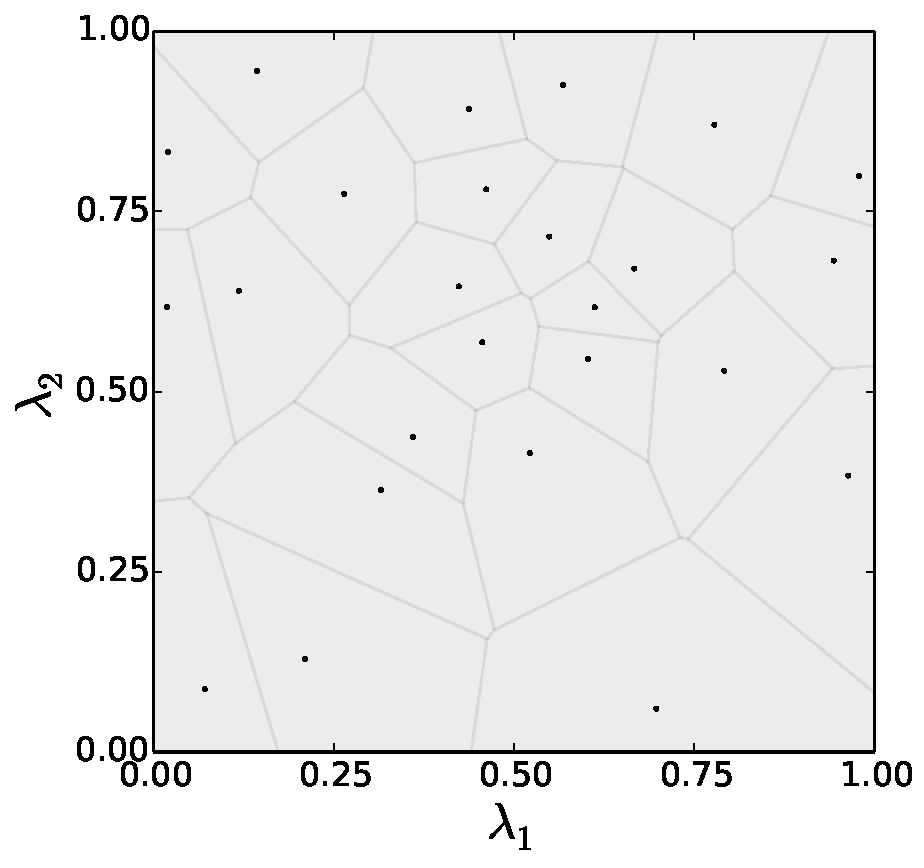
\includegraphics[width=\linewidth]{./images/voronoi_diagram_N25_r0}
	\end{minipage}
	\begin{minipage}{.4875\textwidth}
		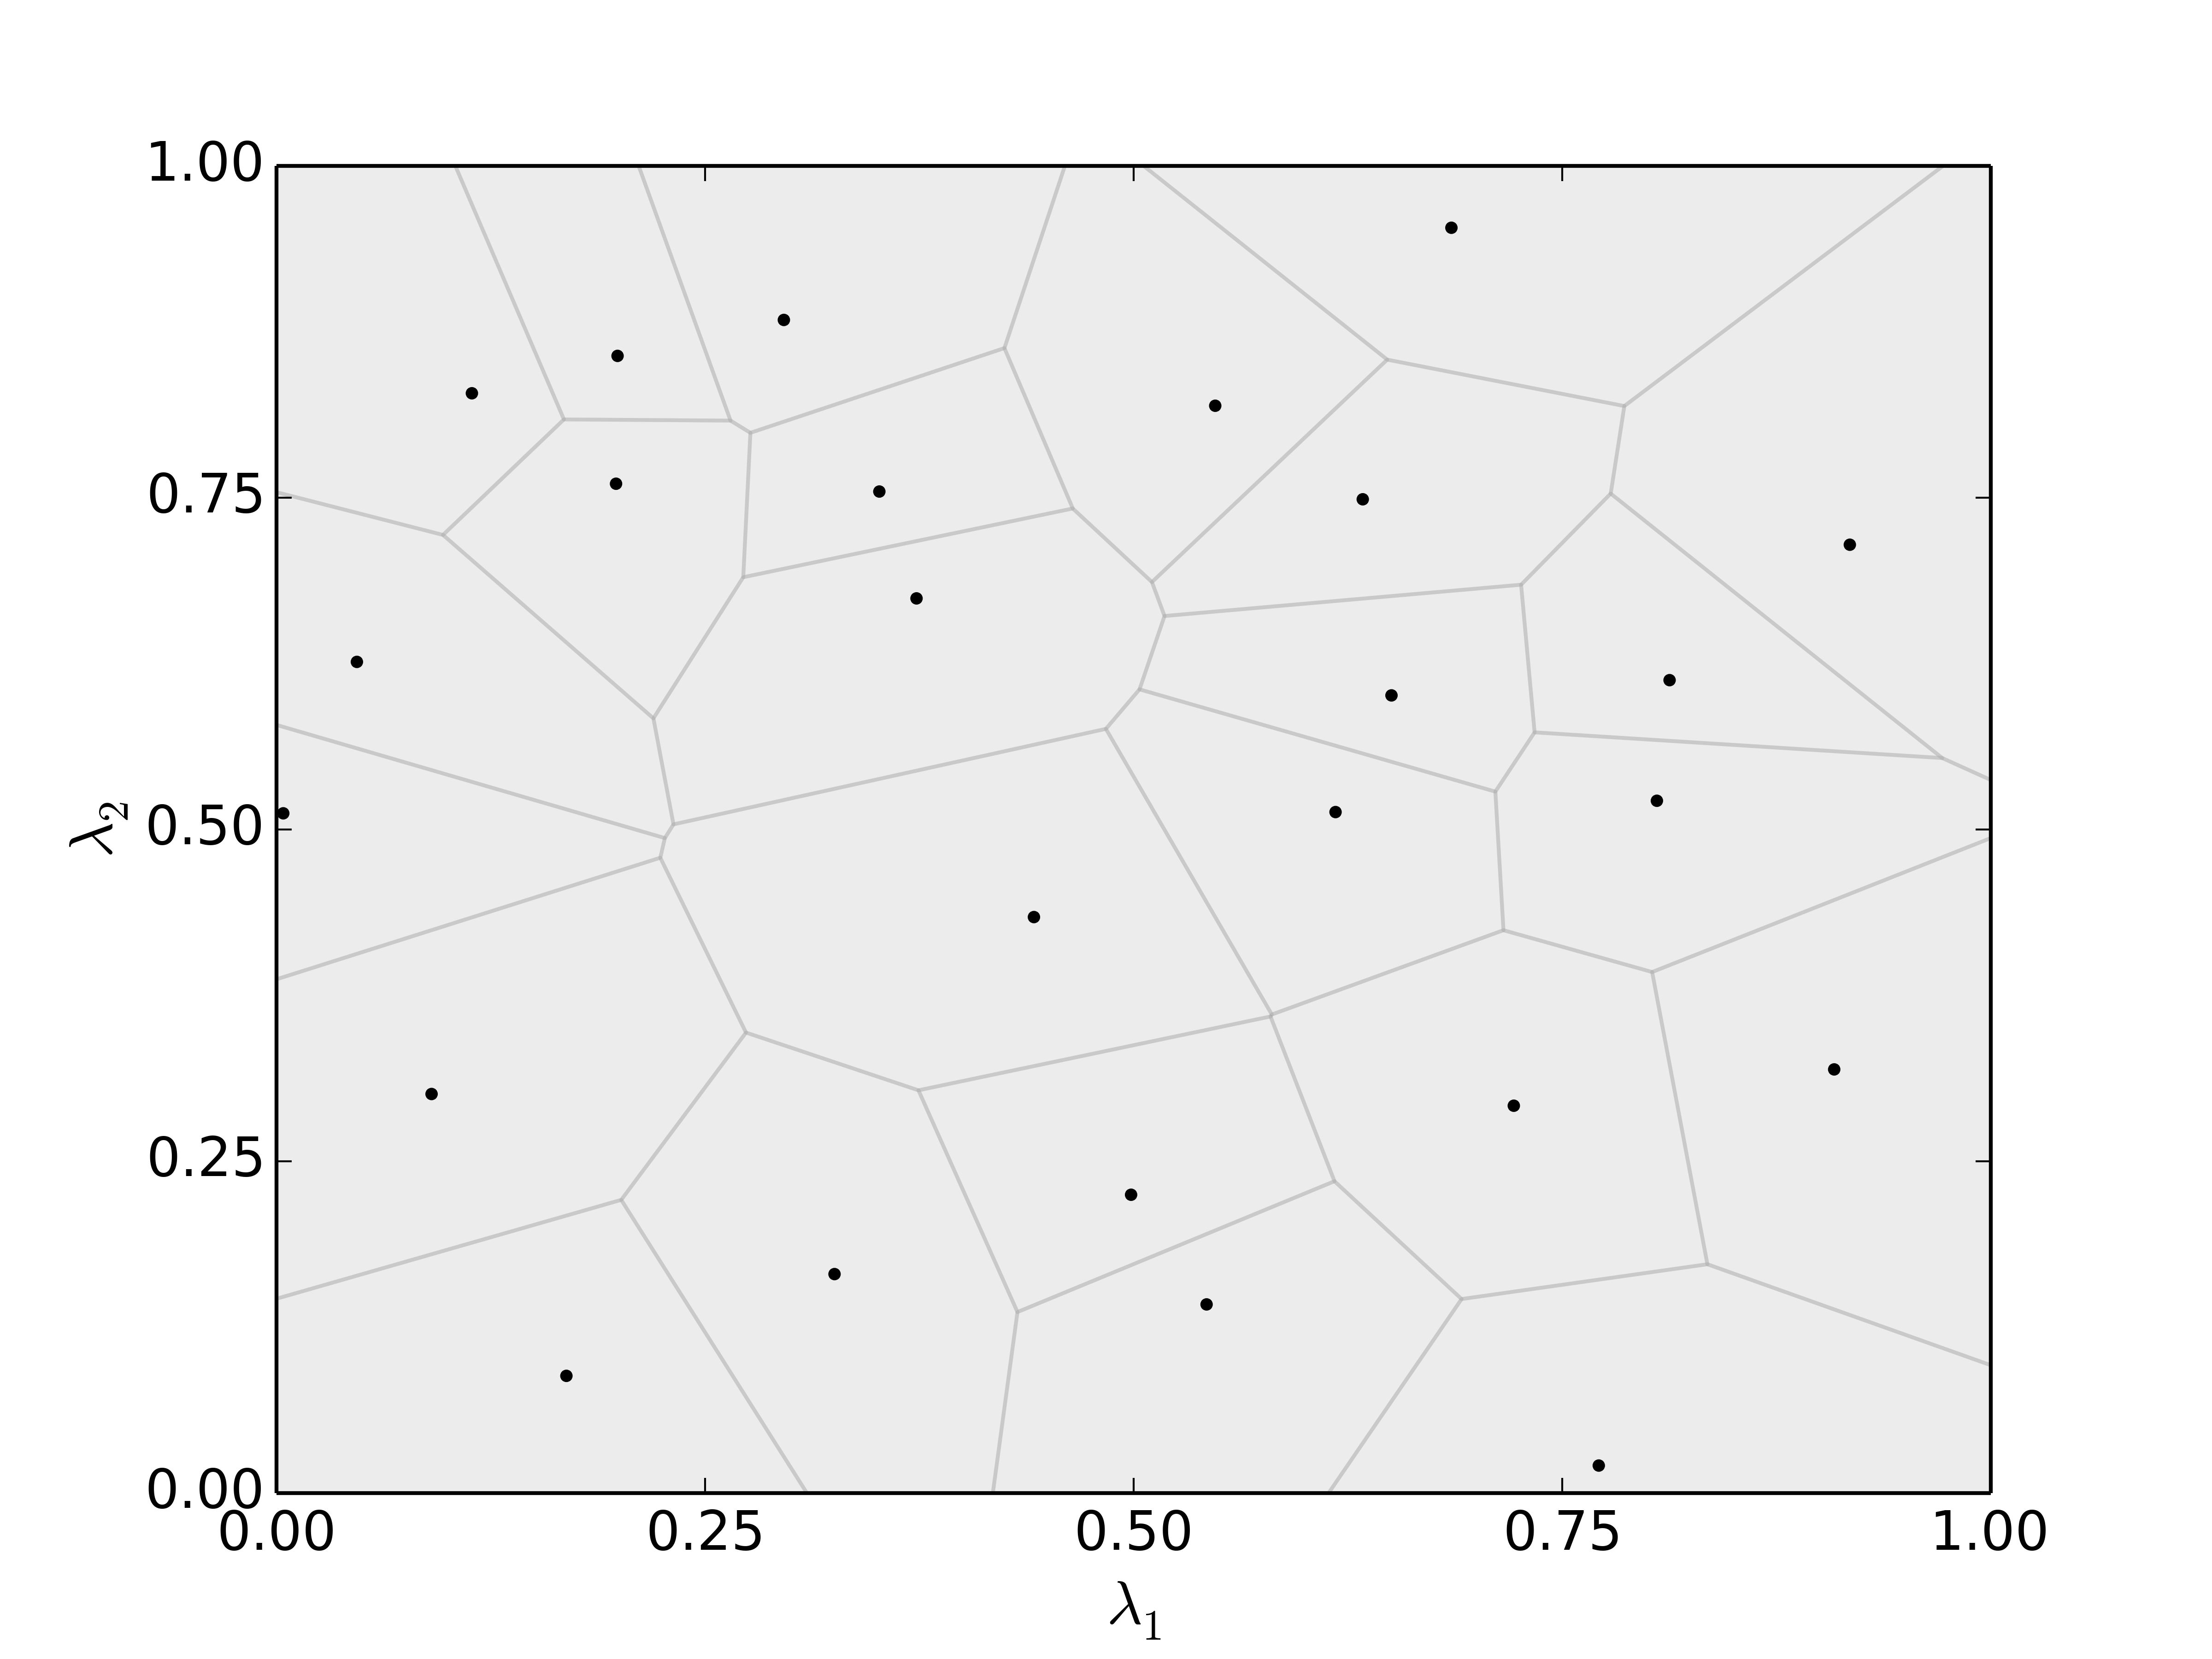
\includegraphics[width=\linewidth]{./images/voronoi_diagram_N25_r10}
	\end{minipage}
\caption{
Two different Voronoi partitions induced by $\nsamps_1 = \nsamps_2 = 25 $ uniform i.i.d.~random samples.
}
\label{fig:voronoi_issues}
\end{figure}


The proof of the following Lemma describes how to ``computationally extend'' {\em any} probability measure defined on a computational algebra to a full $\sa$ $\BB$, which we exploit in Algorithm~\ref{alg:hellinger_disc}.
\begin{lem}
\label{lem:measuresets}
Let $\mu$ be a measure on $(\pspace, \BB_\pspace)$, $\set{\VV^{(j)}}_{j=1}^{\nsamps}$ be a partition of $\pspace$, and $\BB_{\pspace, \nsamps}$ the computational algebra generated by $\set{\VV^{(j)}}_{j=1}^{\nsamps}$.
Assume $\mu (\VV^{(j)}) > 0 \; \forall \; j=1,\hdots, \nsamps$.
Then, there exists a probability measure $\eta$ on $(\pspace, \BB_\pspace)$ such that $\eta(A) = \eta_\nsamps(A) \; \forall \; A\in\BB_{\pspace, \nsamps}$.
\end{lem}
In the proof below, we use $\eta_\nsamps$ and $\mu$ to construct a type of ``discrete'' Radon-Nikodym derivative of $\eta$.
This is motivated by the formal structure of solutions given by Algorithm~\ref{alg:inv_density}.
The proof of Lemma~\ref{lem:measuresets} can be found in Appendix~\ref{app:measuresets}, but the two key equations involved are reproduced here for later reference:

\begin{equation}\label{eq:finiteradon}
f_\nsamps (\param) = \sum_{j=1}^{\nsamps} \frac{\eta_\nsamps (\VV^{(j)}) }{\mu (\VV^{(j)})} \Chi_{\VV^{(j)}} (\param).
\end{equation}

Then, for any $A\in\BB_\pspace$, define

\begin{equation}\label{eq:approxmeasure}
\eta (A) = \int_A f_\nsamps (\param) \, d\mu.
\end{equation}

We note that in practice, $\Chi_{\VV^{(j)}} (\param)$ requires the use of nearest-neighbor computations, but otherwise evaluation of Eq.~\eqref{eq:finiteradon} is straightforward to compute.
With that established, we now present the algorithm used for approximating the distances between pairs of measures (with the computational implementation discussed in \ref{sec:ch03-software}.


\begin{algorithm}
\DontPrintSemicolon
\caption{Total Variation Discretization}
\label{alg:totvar_disc}
Let $(\pspace, B_{\pspace, \nsamps_1}, \eta_{\nsamps_1} )$ and $(\pspace, B_{\pspace, \nsamps_2}, \eta_{\nsamps_2} )$ be given.\\

Construct $f_{\nsamps_1}$ and $f_{\nsamps_2}$ and corresponding $\eta_1, \eta_2$ using Eq.~\eqref{eq:finiteradon} and Eq.~\eqref{eq:approxmeasure}, respectively.

Use Monte Carlo sampling to approximate
$$ d_{TV}(\eta_1, \eta_2) = \int_\pspace f_{\nsamps_1}\lam - f_{\nsamps_2}\lam \, d\mu $$.
\end{algorithm}

Since we now have a way to extend probability measures defined on $(\pspace, \BB_{\pspace, \nsamps})$ to  probability measure on $(\pspace, \BB_{\pspace})$, we can use simple Monte-Carlo approximation schemes to the Hellinger distance between two probability measures defined on two separate computational algebras.
This is demonstrated in Algorithm~\ref{alg:hellinger_disc}.


%%%%%%%%%%%%%%%%%%%%%%%%%%%%%%%%%%%%%%%%%%%%%%%%%%%%%%%%%%%%%%
\subsection{Overview of Examples}
We establish some fundamental properties of solutions to the SIP under different QoI maps in terms of the skewness of the $Q$'s being compared.
We seek an estimated probability measure $\hat{\PP}_\pspace$ on the parameter space to converge (with respect to the metric $d_\text{TV}$) to some reference measure $\PP_\pspace$ as more samples (i.e., model evaluations), $\nsamps$ are used.
Such a reference measure could be either some known distribution taken as truth, or another approximation deemed to be sufficiently resolved for the given application or computational budget (i.e. higher-fidelity model, mesh, or Monte Carlo sample-size).\footnote{However, we could also choose to interrogate the push-forward measures given by propagating the $\hat{\PP}_\pspace$ and $\PP_\pspace$ forward to a data space by a QoI map and taking the distance on the resulting output space.
This would measure the ability of the maps to reconstruct the output probability measure.}

In Figure~\ref{fig:voronoi_sols}, we illustrate the solution to the problem of comparing measures defined on two different (implicitly-defined) $\sa$s shown in Figure~\ref{fig:voronoi_issues}.
By introducing a third set against which both sample sets of size $\nsamps=50$ are compared, we can leverage theoretical results from Lemma~\ref{lem:measuresets} to compare solutions to the SIP under different QoI maps.

\begin{figure}[ht]
\centering
	\begin{minipage}{.275\textwidth}
		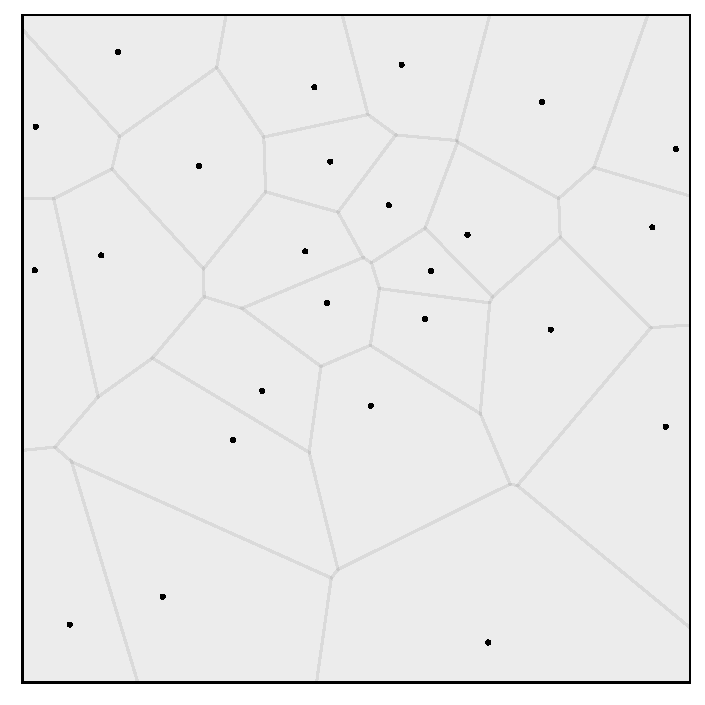
\includegraphics[width=\linewidth]{./images/voronoi_diagrams/voronoi_diagram_N25_r0_no_label}
	\end{minipage}
	\begin{minipage}{.4\textwidth}
		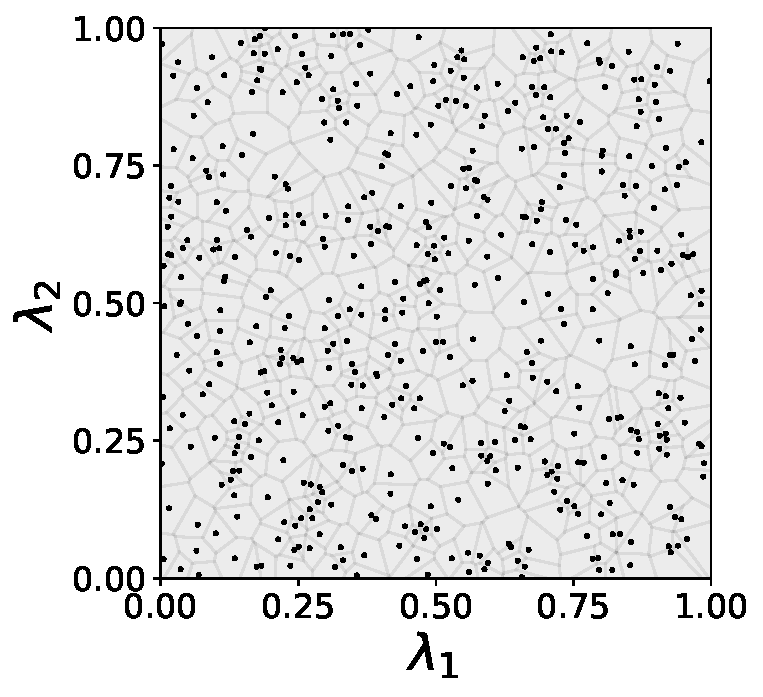
\includegraphics[width=\linewidth]{./images/voronoi_diagrams/voronoi_diagram_N500_r50}
	\end{minipage}
		\begin{minipage}{.275\textwidth}
		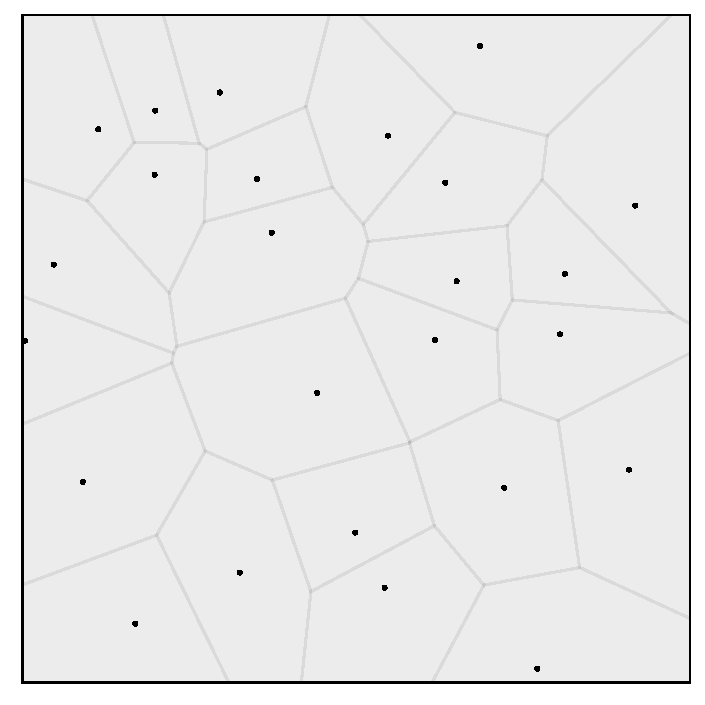
\includegraphics[width=\linewidth]{./images/voronoi_diagrams/voronoi_diagram_N25_r10_no_label}
	\end{minipage}
\caption{
(Left/Right): The two partitions from Figure~\ref{fig:voronoi_issues} will be projected onto a third reference partition (center), in order to compare them on a common $\sa$.
Center: A possibly over-resolved reference sample set, generated using $\nsamps = 500$ uniform i.i.d.~random samples.
}
\label{fig:voronoi_sols}
\end{figure}

To isolate the effect of skewness on the ability to approximate sets with finite sampling, we choose the maps so that they preserve the sizes of sets between $\pspace$ and $\dspace$ under the push-forward measure given in Eq.~\eqref{eq:dataspace_pushforward_measure}.
The sizes of these inverse sets correspond to the average precision of maps $Q$, so we fix the maps to all be equally informative from this perspective; for linear maps, this means they all have the same determinant.

All of our experiments follow the same structure, where $\qspace$ denotes a set of QoI maps under consideration in each example:
\begin{itemize}
\item[[0-a]] Select $\qoi\in\qspace$ and define $\PP_{\dspace_\qoi}$ as a uniform distribution centered on a reference QoI value $Q(\paramref)$ for $\paramref$ taken as the midpoint of $\pspace$.
Note that $\PP_{\dspace_\qoi}$ is exactly discretized with $M=1$ sample, so that
\[
P_{\pspace, 1} = P_\pspace.
\]
\item[[0-b]] Create a regular grid of samples in $\pspace=[0,1]^n$ using $N_{\text{ref},i}$ equispaced points in each dimension.
Set $\bar{N} := \prod N_{\text{ref},i}$.
Since $n$ is small in the numerical examples shown here, we select $N_{\text{ref},i} = 200 \; \forall \; i$ in each example.
\item[[0-c]] Use Algorithm~\ref{alg:inv_density} to construct a reference solution $\PP_{\pspace,\bar{N}}\approx \PP_\pspace$.
\item[[1]] Generate $\set{S_k^{(n)}}_{n=1}^{50}$ sets of uniform i.i.d.~random samples where $N_k = 25, 50, 100, 200, \hdots, 6400$, and $n$ represents the number of repeated trials of a sample size $N_k$.
%, constructing $\set{\set{\VVV_k^{(j)}}_{k=1}^{50}}_{j=1}^{N}$ so that when we compute Total Variation distances on the approximate measures defined on each $\set{\VVV_k^{(j)}}{j=1}{N}$, we can reduce the variance in our expected Total Variation distance values for each instance of $N$. Note that we experimented with using more trials and found the variance in expected Total Variation distances was sufficiently low with as few as twenty trials for the maps under consideration herein.
%\item[[3]] For every trial $T$ and $N$ value (including $\bar{N}$), the reference parameter $\lambda = (\lambda_1, \lambda_2) = (0.5, 0.5)$ is mapped by $Q$ to $\dspace_\qoi = Q(\pspace)$.
%\item[3] A uniform distribution with support $[Q(\lambda_1) - 0.05, Q(\lambda_1) + 0.05] \times [Q(\lambda_2) - 0.05, Q(\lambda_2) + 0.05]$ is defined on $\dspace_\qoi$, representing equal uncertainty in each component of our measured functional values.
\item[[2]] Solve the SIPs using Algorithm~\ref{alg:inv_density} to construct $\set{\PP_{\pspace,M,N}^{(n)}}_{n=1}^{50}$.
\item[[3]] Use $1E5$ i.i.d.~random samples to estimate $\set{d_H^2( \PP_{\pspace,M,N}^{(n)}, \PP_{\pspace,\bar{N}})}_{n=1}^{50}$.
\item[[4]] Average over all trials $n$ for each $N$ to estimate the {\em expected} Total Variation distance for $N$ samples and analyze convergence to $\PP_{\pspace,\bar{N}}$.
\item[[5]] Repeat steps [0-a]--[4] for each $\qoi\in\qspace$ under consideration.
\end{itemize}

\FloatBarrier

\subsection{Rotational Invariance}\label{ex:rotation}
This example shows that if $\qoiA$ is defined by a rotation of $\qoiB$, then the accuracy and convergence rates of $\PP^{(a)}_{\pspace, \ndiscs, \nsamps}$ are identical to $\PP^{(b)}_{\pspace, \ndiscs, \nsamps}$.
We expect this to be true since skewness is rotationally invariant, as we summarize in the following Proposition.
\begin{prop}
The quantity $S_\qoi(\param)$ is invariant under rotations performed on $\qoi$ for any $\param$. \\
\label{prop:rot_invariance}
\end{prop}
\begin{proof}
If we apply a rotation $\qoi$, then the Jacobians $J_{\qoi, \param}$ are also subject to the same rotation at each $\param$.
Since rotations are unitary operators, the norms given in Eq.~\eqref{eq:skewness} used to define skewness are unaffected.
\end{proof}

\begin{figure}
\begin{minipage}{.5\textwidth}
\begin{table}[H]
\begin{tabular}{ c | c | c | c }
\nsamps & $\qoiA$ & $\qoiB$ & $\qoiC$\\ \hline \hline
$200$ & $2.18E-01$ & $1.97E-01$ & $2.19E-01$\\ \hline

$400$ & $1.60E-01$ & $1.70E-01$ & $1.51E-01$\\ \hline

$800$ & $1.09E-01$ & $1.14E-01$ & $1.09E-01$\\ \hline

$1600$ & $7.43E-02$ & $7.76E-02$ & $7.53E-02$\\ \hline

$3200$ & $5.51E-02$ & $5.53E-02$ & $5.31E-02$\\ \hline

$6400$ & $4.19E-02$ & $4.09E-02$ & $4.19E-02$\\ \hline
\end{tabular}
\end{table}
\end{minipage}
\begin{minipage}{.45\textwidth}
		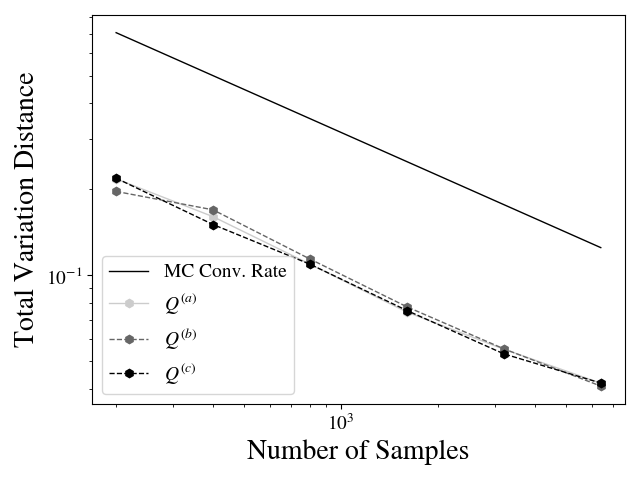
\includegraphics[width=\linewidth]{./images/Plot-orth-reg_BigN_40000_reg_M_1_rand_I_100000.png}
\end{minipage}
\caption{The results of $d^2_\text{TV}(\PP_{\pspace, \ndiscs, \nsamps}, \PP_{\pspace, \bar{\nsamps}})$ for three maps generated by random rotations of orthogonal linear maps.}
\label{fig:M1orth}
\end{figure}

To demonstrate this Lemma numerically, we define the space of QoI maps $\qspace = \set{ \qoiA , \qoiB, \qoiC }$, where all three are linear maps with the same local skewness $S_\qoi (\param) = 1 \; \forall \param \in \pspace$.
The map $\qoiA$ is the identity and the other two, $\qoiB$ and $\qoiC$ are rotations of $\qoiA$ by randomly chosen angles.
Following the algorithmic outline above, we perform a convergence study to $\PP_{\pspace,\bar{\nsamps}}$ with results summarized in Figure~\ref{fig:M1orth}.
The convergence rates and expected errors in the SIPs associated with each of these maps are virtually indistinguishable.
In light of Proposition~\ref{prop:rot_invariance} and these numerical results, we conclude that the accuracy of the numerical solution to the SIP is invariant under rotations to the QoI map.

\FloatBarrier

%%%% 2D Skewness Example %%%%%% 
\subsection{Impact of Skewness on Accuracy}\label{ex:skewness}
In this example, we demonstrate the key point of this study: the magnitude of skewness between QoI impacts accuracy by orders of magnitude, and thus in optimizing the choice of a QoI map, it is in our interest to pursue the minimization of skewness. 
This is especially true in problems where the number of random samples we are permitted to use is constrained by the computational cost of model evaluations.

%Thus, any map can be thought of as a piecewise-defined linear map, and the results we present in this example, while applying to all of $\pspace$ in these cases, can be applied solely to the support of each local linear approximation.
%Capturing the geometry of sets (improving accuracy) on each of these subdomains thus guarantees a desired result on the entirety of the domain. 

To illustrate this point, we first define the linear maps 
\begin{equation}\label{eq:qmap2}
\qspace_S := \left \lbrace Q^{(s)} =  \mat{cc}{1 & 0 \\ \sqrt{s^2 - 1}& 1 } \right \rbrace_{s\in S},
\end{equation}
for $S=\set{1,2,4}$ because they allow us to control the global skewness (since it is equal to local skewness in a linear map) while preserving the measures of sets between $\pspace$ and $\dspace$. 
More specifically, the support of the solution to the SIP associated with each QoI map has equal $\mu_\pspace$-measure, which isolates the impact of accuracy solely to the skewness of the QoI map.
We show what the component row vectors of these maps in Figure~\ref{fig: skewmapvecs} and note the skewness is determined by the ratio of the magnitude of the black line to its projection onto the vertical axis (and each of these projects directly on to the unit vector).  
The skewness of these maps is given by the index $s$, so $Q^{(1)}$ is $1$, the skewness of $Q^{(2)}$ is $2$, and $S_{Q^{(4)}} = 4$.

The maps chosen for this example are expository ones that provide valuable insight despite their simplicity. 
For example, when solving many physics-based problems, local linear approximations are often used to simplify model evaluation and guide optimization procedures.


\begin{figure}[h]
	\begin{minipage}{.3\textwidth}
		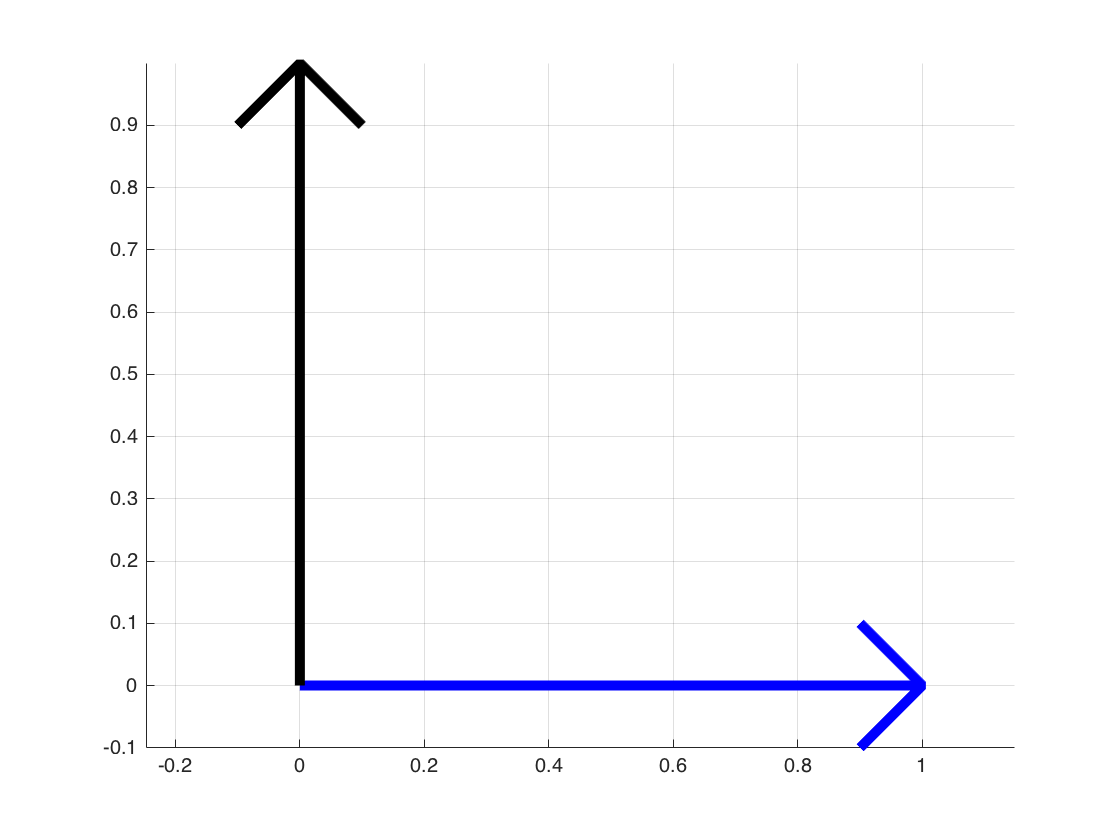
\includegraphics[width=\linewidth]{./images/vector_a.png}
	\end{minipage}
	\begin{minipage}{.3\textwidth}
		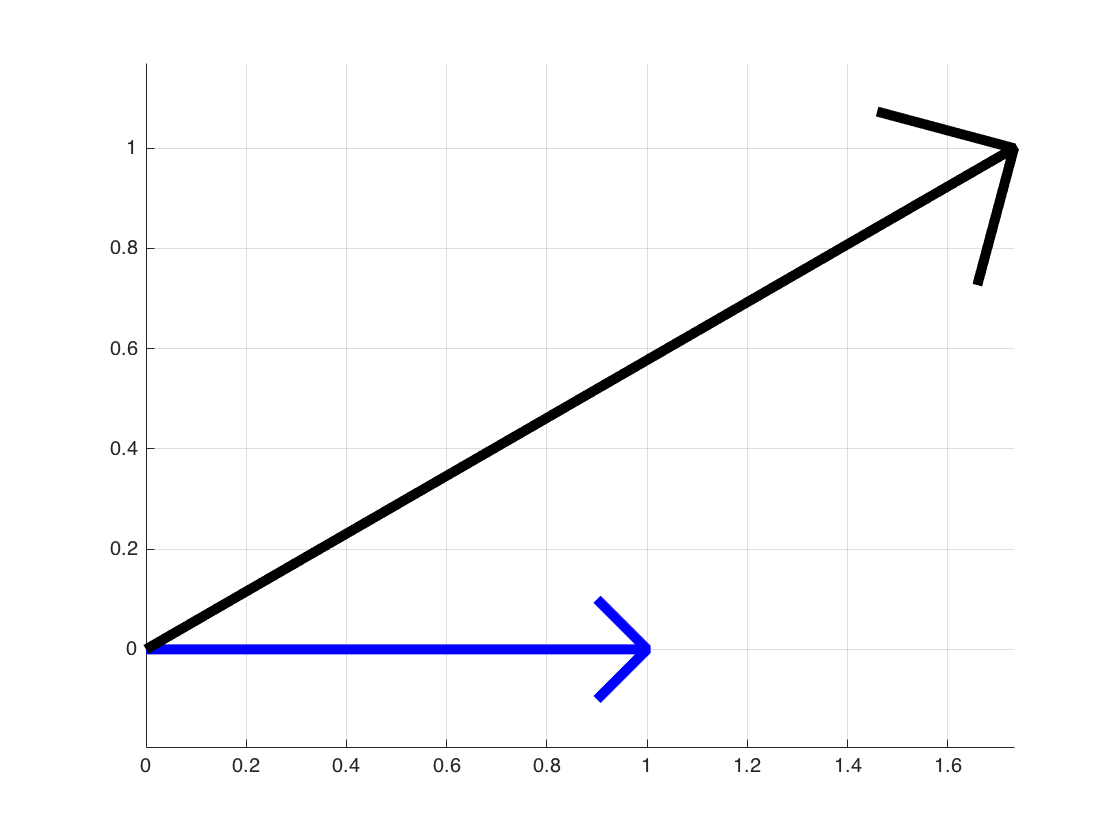
\includegraphics[width=\linewidth]{./images/vector_b.png}
	\end{minipage}
	\begin{minipage}{.3\textwidth}
		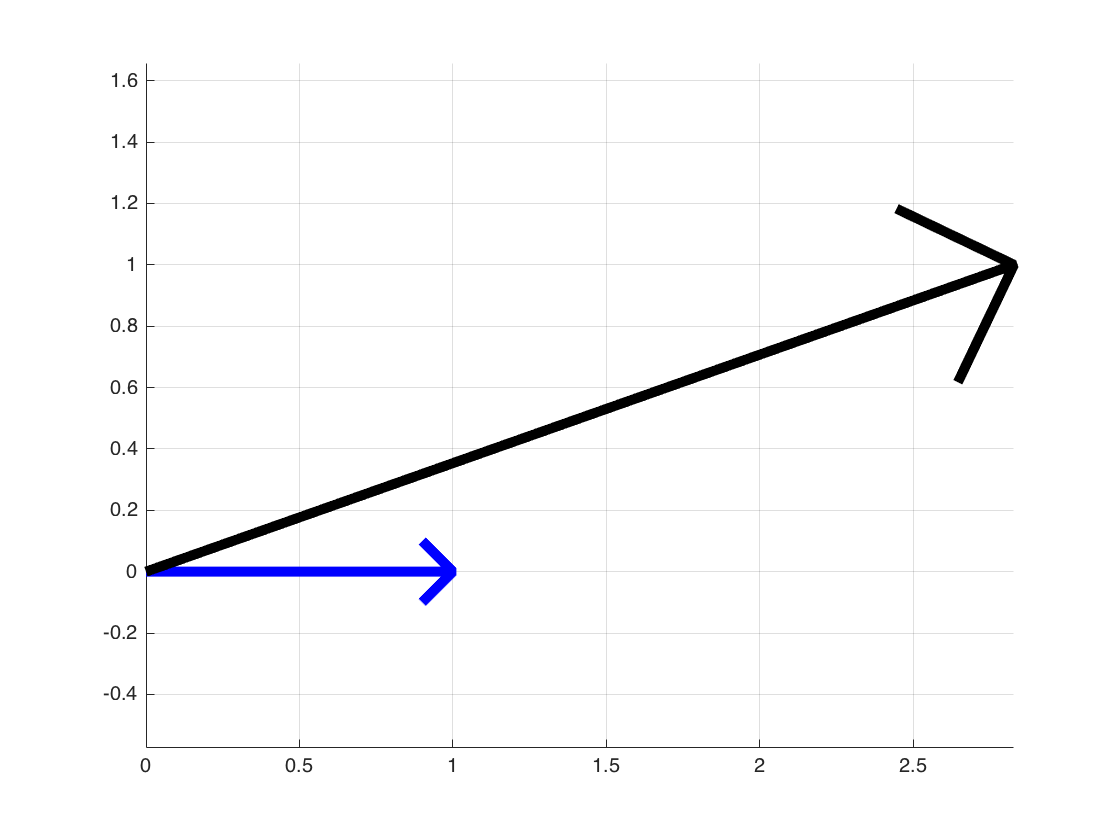
\includegraphics[width=\linewidth]{./images/vector_c.png}
	\end{minipage}
\caption{(Left to right):  The component row-vectors of $Q^{(1)}$, $Q^{(2)}$, and $Q^{(4)}$. Our linear maps take $\RR^2$ to $\RR^2$ and can be visualized graphically as the component row-vectors of the matrices representing the transformation. The first row is highlighted in blue. The skewness is then simply equal to the reciprocal of the inverse sine of the angle between these vectors. }
\label{fig: skewmapvecs}
\end{figure}


\begin{figure}
\begin{minipage}{.5\textwidth}
\begin{table}[H]
\begin{tabular}{ c | c | c | c }
N & $Q^{(1)}$ & $Q^{(2)}$ & $Q^{(4)}$\\ \hline \hline
$200$ & $1.35E-01$ & $2.03E-01$ & $3.12E-01$\\ \hline 
 
$400$ & $9.96E-02$ & $1.47E-01$ & $2.15E-01$\\ \hline 
 
$800$ & $7.19E-02$ & $1.04E-01$ & $1.53E-01$\\ \hline 
 
$1600$ & $5.27E-02$ & $7.49E-02$ & $1.10E-01$\\ \hline 
 
$3200$ & $3.70E-02$ & $5.25E-02$ & $7.52E-02$\\ \hline 
 
$6400$ & $2.76E-02$ & $3.86E-02$ & $5.54E-02$\\ \hline 
\end{tabular}
\end{table}
\end{minipage}
\begin{minipage}{.45\textwidth}
		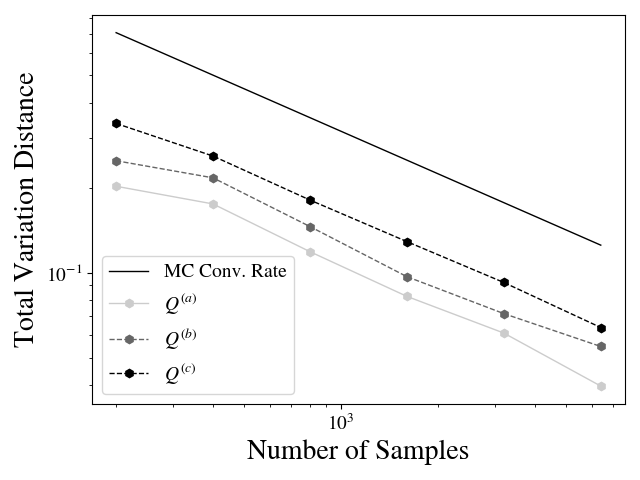
\includegraphics[width=\linewidth]{./images/Plot-reg_BigN_40000_reg_M_1_rand_I_100000}
\end{minipage}
\caption{The results of $d^2_H(\PP_{\pspace, M, N}, \PP_{\pspace,\bar{N}})$.}
\label{fig:M1_2d}
\end{figure}

We see in Figure~\ref{fig:M1_2d} that skewness has a very direct impact on the number of samples required to achieve a particular value for the Hellinger distance. 
We can see that the measure induced by $Q^{(1)}$ requires fewer than half the number of samples to be as accurately resolved as $Q^{(2)}$ does. 
The effect is even more pronounced when compared against $Q^{(4)}$.
It appears that if the ratio of skewness between two maps is 2, then the more-skewed map will require at least twice as many random samples to approximate the set on a a well-resolved discretization with the same error tolerance.

This provides a strong motivation for minimizing skewness and reinforces the results from \cite{BPW_2015}, where it was demonstrated that a similar relationship existed in the number of samples required to remove error in inverse set approximations quantified by the $\mu_\pspace$-measure of the {\em symmetric difference} of the inverse sets.




%%%% 3D Skewness Example %%%%%%

\subsection{Dependence on Dimension}\label{ex:3dmap}
To further illustrate that relationship between skewness and accuracy holds as we move towards higher dimensions, we extend the numerical investigation to a three--dimensional parameter space.
Generally, we have fewer QoI than number of uncertain model parameters, so we assume that the potential QoI maps are defined by the $2\times 3$ matrices
\begin{equation}\label{eq:qmap3}
\qspace_S := \left \lbrace \qoi^{(s)} =  \mat{ccc}{1 & 0 & 0\\ \sqrt{s^2 - 1}& 1 & 0} \right \rbrace_{s\in S}.
\end{equation}
Here, as in the previous example, the index $s$ indicates the magnitude of skewness.
Furthermore, the results of Example~\ref{ex:rotation} justify the restriction of the maps to this form since any linear map of skewness $s$ is simply a rotation of maps of this form.

%Now, the generalized contours for inverses of maps from $\RR^3 \to \RR^2$ will be isomorphic to 2\--dimensional contour events in that the inverse sets will be columns in 3\-space orthogonal to the aforemntioned plane.
%
%IMAGE DEMONSTRATING THIS WOULD HELP.
%We define
%
%which is just the map from \eqref{eq:qmap2} appended with zeros in the third column.
%We make this choice solely for convience and are justified in doing so owing to Proposition~\ref{prop:rot_invariance} and the fact of generalized contours of maps from $\RR^3 \to \RR^2$ being parallel columns.
%The rotational invariance naturally extends to the third dimension.

%We note that $\bar{N}$ is much higher since we kept the convention of 200 grid cells per dimension in our reference.
%However, we kept the same number of random samples $N$, so we should expect higher errors due to the overresolved regular grid.
%Fortunately, we find that the results still generalize.
%We present the case where $M=1$:

\begin{figure}[h]
\begin{table}[H]
\begin{tabular}{ c | c | c | c }
\nsamps & $\qoiA$ & $\qoiB$ & $\qoiC$\\ \hline \hline
$200$ & $3.33E-01$ & $4.56E-01$ & $6.10E-01$\\ \hline

$400$ & $2.78E-01$ & $3.51E-01$ & $4.97E-01$\\ \hline

$800$ & $2.19E-01$ & $2.95E-01$ & $4.10E-01$\\ \hline

$1600$ & $1.72E-01$ & $2.37E-01$ & $3.35E-01$\\ \hline

$3200$ & $1.36E-01$ & $1.89E-01$ & $2.64E-01$\\ \hline

$6400$ & $1.09E-01$ & $1.47E-01$ & $2.09E-01$\\ \hline
\end{tabular}
\end{table}

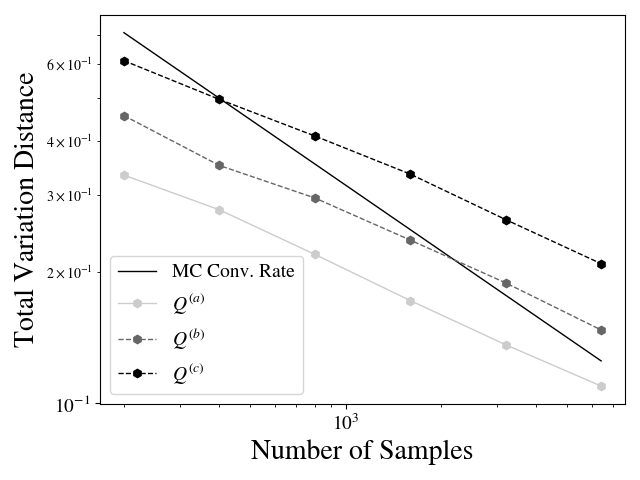
\includegraphics[width=0.45\linewidth]{./images/Plot-reg_BigN_8000000_reg_M_1_rand_I_100000.png}

\caption{The results of $d^2_\text{TV}(\PP_{\pspace, \ndiscs, \nsamps}, \PP_{\pspace, \ndiscs, \bar{\nsamps}})$ for $\ndiscs = 1, \bar{\nsamps} = 8,000,000$, with $a, b, c = 1, 2, 4$ in three dimensions.}
\label{fig:M1_3d}
\end{figure}
\FloatBarrier
In Figure~\ref{fig:M1_3d}, it appears that the effect of skewness is even more pronounced in higher dimensions, and that the number of samples required to achieve similar levels of accuracy between two maps with a ratio of skewness 2 is now quadrupled.
The analysis of \cite{BGE+15} suggested a dependence of accuracy related to the skewness raised to a power related to the dimension of the data space.

%%%%%%%%%%%%%%%%%%%%%%%%%%%%%%%%%%%%%%%%%%%%%%%%%%%%%%%%%%%%%%

% \section{Accuracy of Sample-Based Inversion}\label{sec:ch03-sample}

How does the new approach compare? What role does the KDE play in the error?
Focus on linear problems. One or two examples (perhaps use that skew-map with 1 and 2 and 4).

%%%% Sample-Based Skewness Example %%%%%%

\subsection{A Sample-Based Solution}\label{eq:sampleskew}

Here we solve the problems in Examples~\ref{ex:skewness} and~\ref{ex:3dmap}, except in the framework of the Sample-Based Inversion outlined in \ref{sec:ch02-sample}.
Effect of Skewness appears to be mitigated.
\vfill{10in}

%%%%%%%%%%%%%%%%%%%%%%%%%%%%%%%%%%%%%%%%%%%%%%%%%%%%%%%%%%%%%%

\
\section{Numerical Results and Analysis}\label{sec:ch03-examples}


We have an interest in understanding what values of $\nsamps$ would be appropriate provided we want to resolve $d(\PP_{\pspace, \ndiscs, \nsamps}, \PP_{\pspace, \ndiscs})$ to some desired level of accuracy, below some tolerance so that Equation~\eqref{eq:objective} is effectively satisfied if
\begin{equation}\label{eq:newobjective}
d(\PP_{\pspace, \ndiscs, \nsamps}, \PP_{\pspace,\ndiscs}) < \tau,
\end{equation}
where $\tau$ is some designated tolerance.

Recall that this discussion of error is in reference to some fixed $\qoi\in\qspace$ to which Algorithm~\ref{alg:inv_density} is applied.
The inequality presented in Eq.~\eqref{eq:set-triangleineq} holds for probability measures induced by any map in $\qspace$, though we obscure the dependence on $\qoi$ for the time being.
To this end, we introduce notation of the form $\PP_{\pspace, \ndiscs, \nsamps}^{\qoi}$ when we want to distinguish between measures constructed from inverting a particular map $\qoi\in\qspace$.

The reason for this is because as the work of (cite: Butler AWR) has shown, the choice of $\qoi$ will influence the number of model solutions necessary to accurately solve the SIP.
Different choices for $\qoi$ may lead to radically different values for $\nsamps$ in order to achieve the same bound on $d(\PP_{\pspace, \ndiscs, \nsamps}, \PP_{\pspace, \ndiscs})$, and it is the goal of this work to explore this relationship.

The analysis of this problem differs significantly from the ones in (cite: butler, mattis), which bound errors in probability of estimating sets $A\in\pborel$.
By phrasing our analysis in terms of metrics (discussed more in Section~\ref{sec:metrics}), we may be able to answer more broadly generalizable questions about error, including those regarding convergence rates and global accuracy of our estimates.


Total Variation\subsection{Example: Thermal Conductivity on a 1D Heat Rod}\label{ex:heat-set-sample-accuracy}
In this example we demonstrate that where measurements are taken have an impact on the ability to accurately approximate the solution to the SIP.
In addition, we show that when nonlinearities are present in the map, the location of the true parameter distribution or value have an equally compelling impact.
This impact is due to the fact that skewness is a local property that is averaged out over $\pspace$ to give an average measure of geometrically distinct information.
We set up the following nonlinear problem involving heating a theoretical 1-D rod to make these takeaways clear.

Consider the one-dimensional heat equation with homogeneous Neumann boundary conditions on the unit interval:

\begin{equation}
\begin{split}
\rho c \frac{\partial T}{\partial t} = \nabla \cdot ( \kappa \nabla T) + f(x), \quad & x\in (0,1), t\in (0,1) \\
f(x) = A e^\frac{- (x-0.5)^2}{w} \Chi_{[0,0.5]}(t)
\end{split}
\end{equation}
\emph{Alternative setup: }

\begin{equation}
\begin{cases}
\rho c \frac{\partial T}{\partial t} = \nabla \cdot ( \kappa \nabla T) + f(x,t), & \text{if } x\in \Omega \\
\frac{\partial T}{\partial \vec{n}} = 0 & \text{if } x\in \partial \Omega
\end{cases}
\end{equation}
where $\Omega = (0,1)\times (0,1)$ is the space-time interior and $f(x,t) = A e^\frac{- (x-0.5)^2}{w} \Chi_{[0,0.5]}(t)$.

Here, we interpret the following problem as heating the middle of an infinitesimally thin unit-length rod for half a second with a heat-source modeled by a Gaussian curve with amplitude $A=50$ and variance of $w=0.05$.
This heat source is turned on at the beginning of the experiment and turned off halfway through the 1-second duration.

The rod is subdivided in two, and each half has an uncertain thermal diffusivity $\kappa \in [0.01, 0.2]$.
This yields a two-dimensional parameter space $\param = (\param_1, \param_2) \in [0.01, 0.2]^2$, where $\param_1$ represents the thermal diffusion on the left-half and $\param_2$ is the $\kappa$ for the right half.

Two measurement locations along the rod are used for taking a measurement
We assume a uniform density for each observation with a side--length of $0.1$ and attempt to identify a set which contains our true reference value of $\paramref = (0.15, 0.05)$.

The quantities of interest we study are four point-evaluations of the state variable, at spatial location 0.25, 0.51, 0.67, and 0.98 along the rod.
Choosing any pair of them for the inversion yields six possible quantities of interest maps.
As before, we demonstrate that some choices appear to have advantages over others.

From the prior examples, we would suspect that choosing the QoI map with lower skewness results in lower Total Variations.
However in the earlier experiments we utilized maps that inverted into sets of identical size, which is not the case in this nonlinear example; each QoI map scales sets differently depending on the location in the parameter space.
To isolate this scaling effect, we attempt to compare QoIs that invert into sets of similar size \emph{on average} but have differing average skewness.

This is what motivated our specific choice of spatial locations at which to measure the state variable $T$.
Our first QoI $\qoiA$ uses measurements at 0.25 and 0.51, and has average skewness of 1.08, and our second $\qoiB$ uses measurements at 0.67 and 0.98, with average skewness 1.56.
While we would have liked to use a map with average skewness of 2 for a more similar comparison to the prior examples, this was the best range we could find where the maps inverted into sets of comparable size on average\footnote{average local scaling is $1.99$ for $\qoiA$ and $2.19$ for $\qoiB$.}.

Owing to the nonlinearity of the problem, the Total Variations between reference and estimated probability measures now have an inherent dependence on the location of the point $\param$ in the parameter space.
We ran the simulations for a regular $3\times3$ grid exploring the interior of the parameter space and present two of the nine reference points that illustrate the differences in the nonlinear case from the linear examples.
Most notably, the location of truth will impact our ability to approximate the solution to the SIP.

In the two-dimensional data spaces $\dspaceA$ and $\dspaceB$, our uncertainty is a uniform box centered at $\qoiA(\paramref)$ with side-lengths of 0.1.
When $\paramref$ is the bottom-left corner of our $3\times3$ grid, the two maps produce very different results, with $\qoiA$ outperforming $\qoiB$ in a similar manner as we saw in the linear examples (see Fig.~\ref{fig:NLbotleft}).
When $\param_{\text{ref}}$ is in the upper-center of the grid, the inverse images are similar, as shown in Fig.~\ref{fig:NLtopmid}, and so which map to use forinversion into this part of the parameter spaces is not a clear choice. We might even be tempted to use the more-skewed (on average) map since it inverts into a set with smaller support.


\begin{figure}[h]
  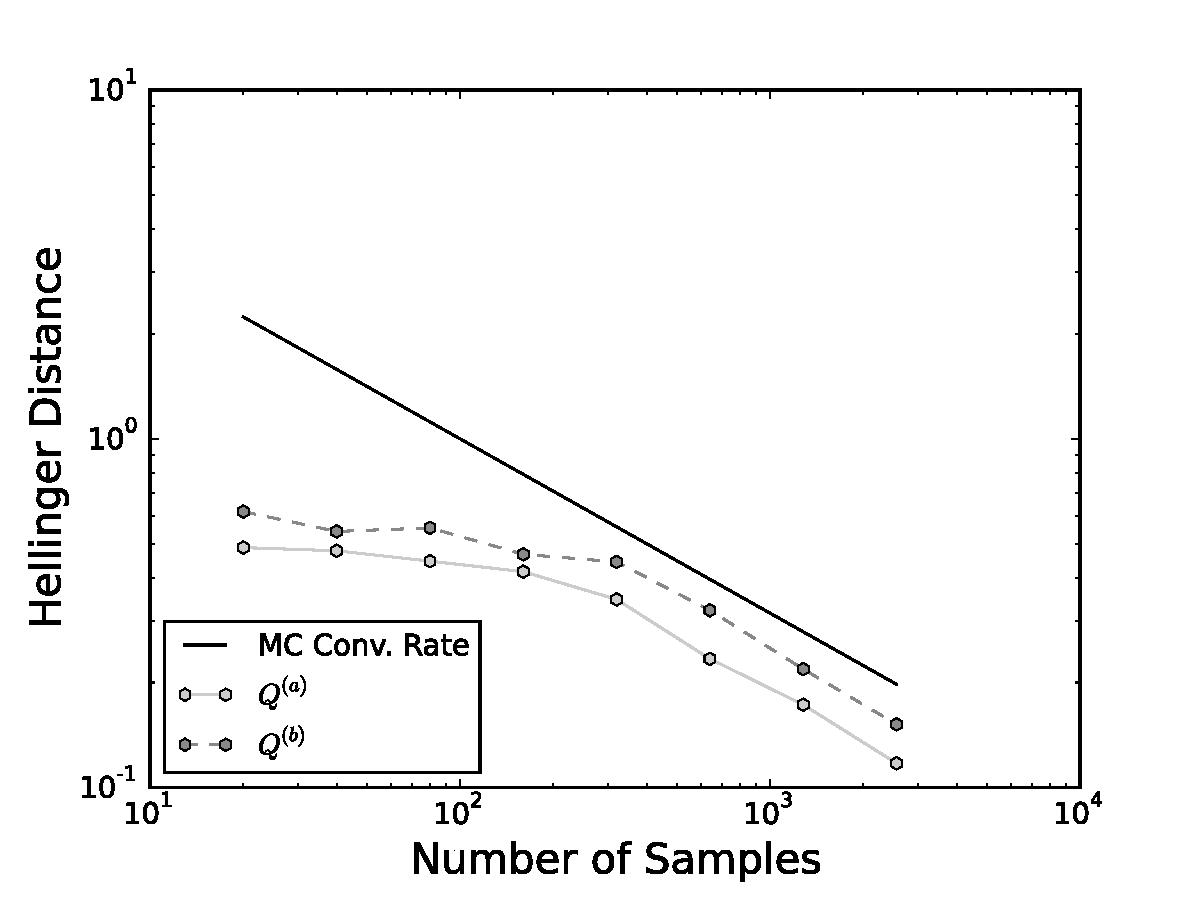
\includegraphics[width=\linewidth]{./images/pt0Plot-reg_BigN_40000_reg_M_1_rand_I_100000}
  \caption{Convergence in TV metric for the bottom left reference value in a 3x3 grid in $\pspace$. There is a notable difference in the accuracy of the measure recovered depending on which QoI map is used.}
  \label{fig:NLbotleft}
\end{figure}

\begin{figure}[h]
  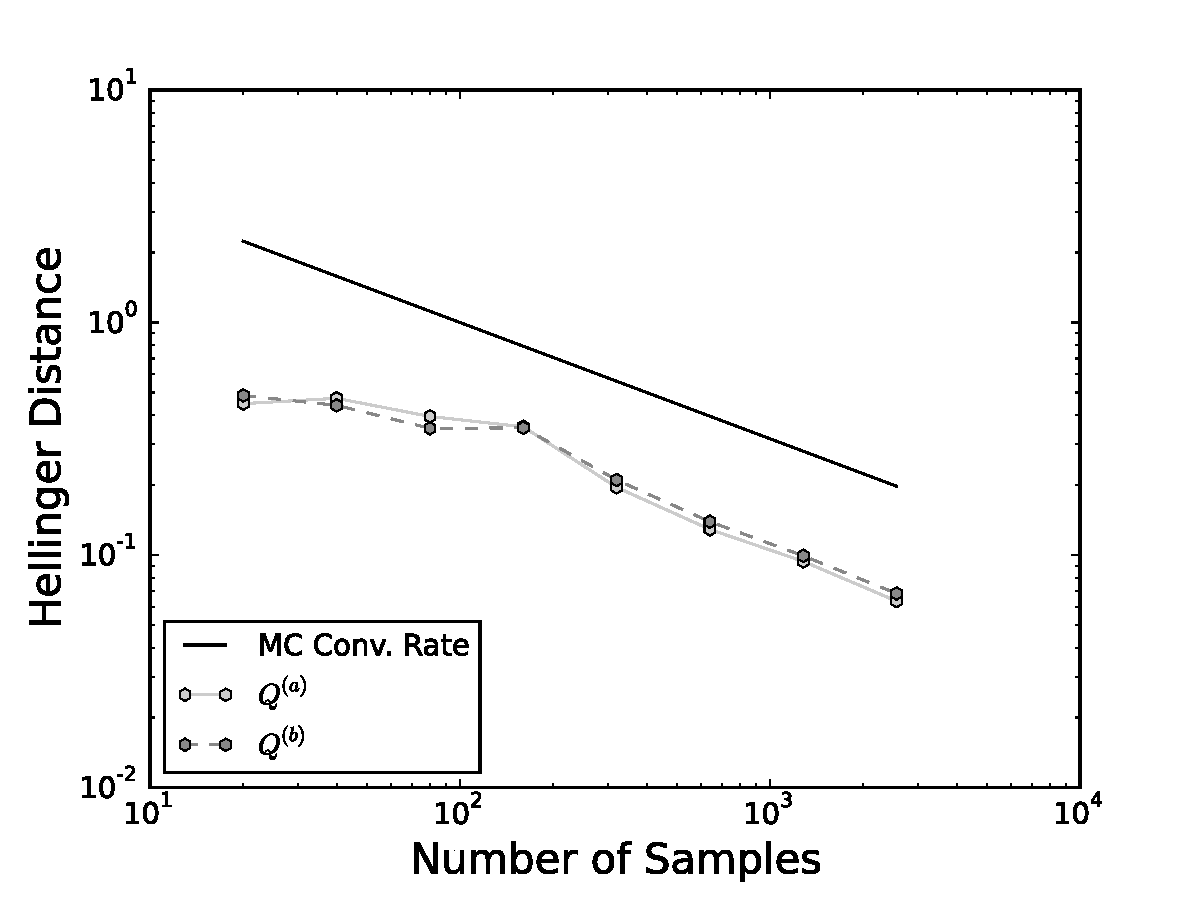
\includegraphics[width=\linewidth]{./images/pt5Plot-reg_BigN_40000_reg_M_1_rand_I_100000}
  \caption{Convergence in TV metric for the top-middle reference value in a 3x3 grid in $\pspace$. For this value of truth, there is no distinguishable difference between the solutions that come from using either QoI map. The location in parameter space of truth will impact how sensitive experimental designs are to approximation errors in limited exploration of $\pspace$.}
  \label{fig:NLtopmid}
\end{figure}


Of the nine reference $\param$'s we studied, $\qoiA$ yielded no considerable advantage in terms of the number of samples required to approximate the inverse images in three cases (the plots were similar to that in the right of Fig.~\ref{fig:NLHD}).
In three cases, $\qoiA$ performed better than $\qoiB$, (somewhere between the two figures in Fig.~\ref{fig:NLHD}).
In two cases, $\qoiA$ performed better than  $\qoiB$, as in the left of Fig.~\ref{fig:NLHD}.
In one case (with $\param$ in the bottom right corner), the difference was even more dramatic ($\qoiA$ yielded similar Total Variations with less than a fourth the samples).

\begin{figure}
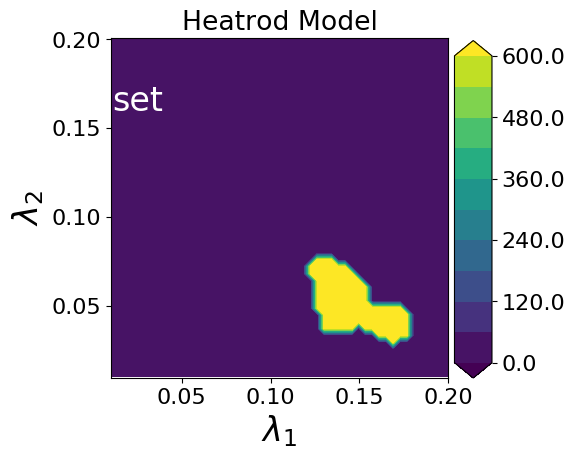
\includegraphics[width=.45\linewidth]{examples/fig_heatrod_q1/HeatrodModel--set_N50_em.png}
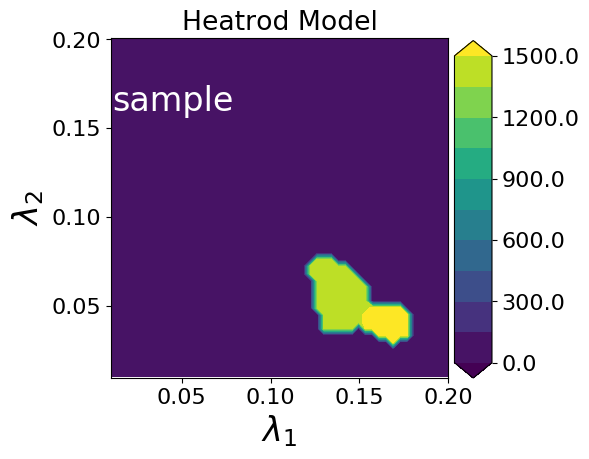
\includegraphics[width=.45\linewidth]{examples/fig_heatrod_q1/HeatrodModel--sample_N50_mc.png}

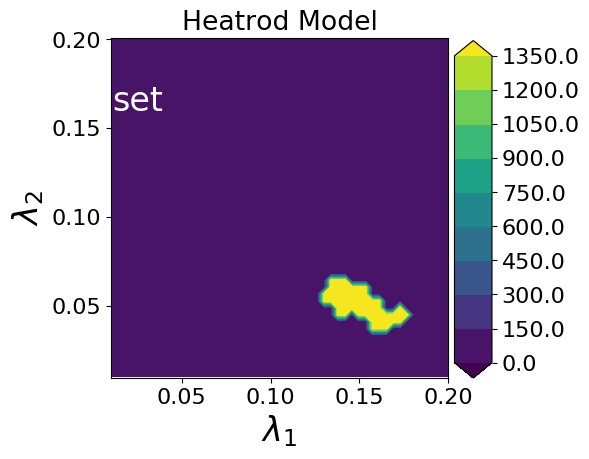
\includegraphics[width=.45\linewidth]{examples/fig_heatrod_q1/HeatrodModel--set_N500_em.png}
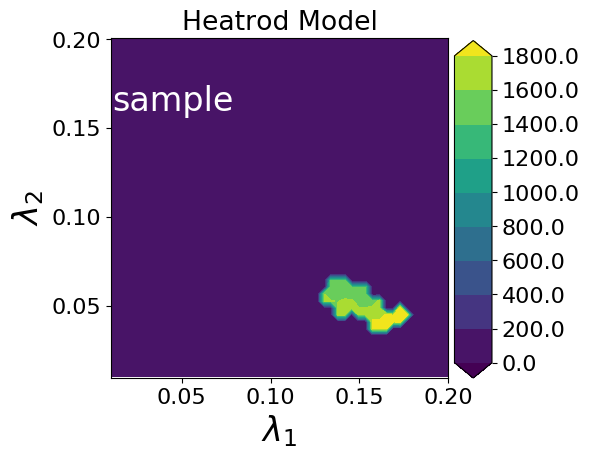
\includegraphics[width=.45\linewidth]{examples/fig_heatrod_q1/HeatrodModel--sample_N500_mc.png}

\caption{The inverse image of the reference measure for $\qoiA$ for $\nsamps = 50$ (top) and $\nsamps = 500$ (bottom). }
\label{fig:heatrod-convergence-a}
\end{figure}

\begin{figure}
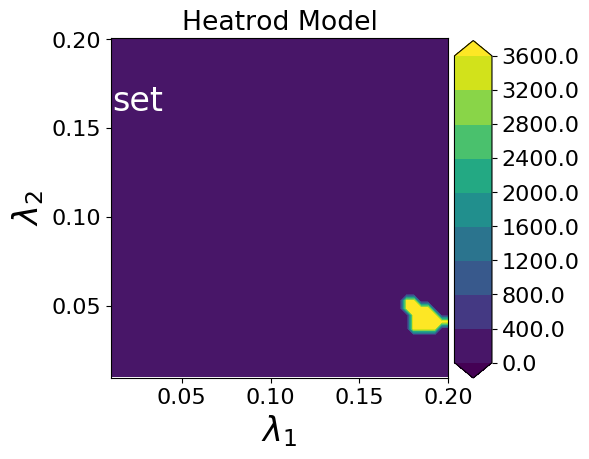
\includegraphics[width=.45\linewidth]{examples/fig_heatrod_q2/HeatrodModel--set_N50_em.png}
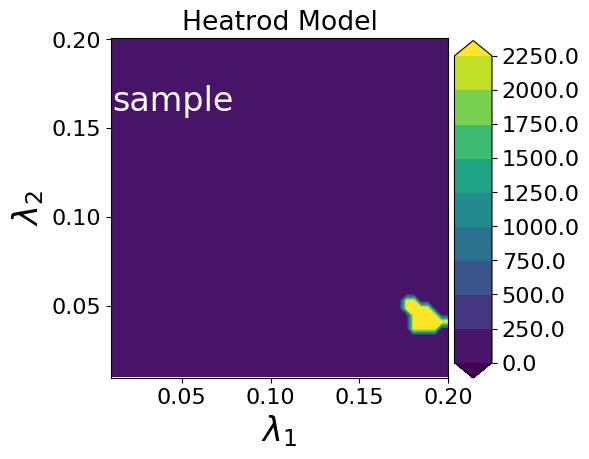
\includegraphics[width=.45\linewidth]{examples/fig_heatrod_q2/HeatrodModel--sample_N50_mc.png}

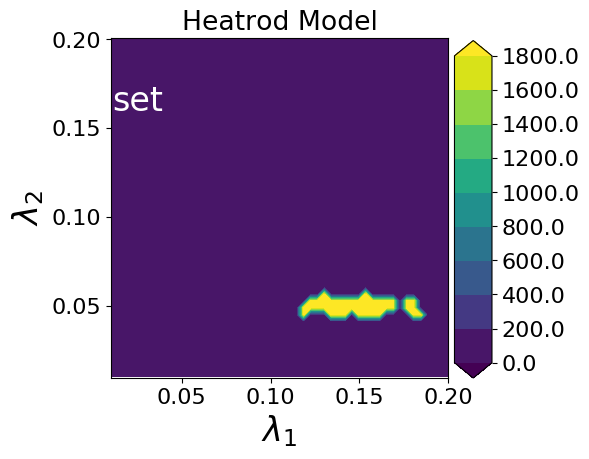
\includegraphics[width=.45\linewidth]{examples/fig_heatrod_q2/HeatrodModel--set_N500_em.png}
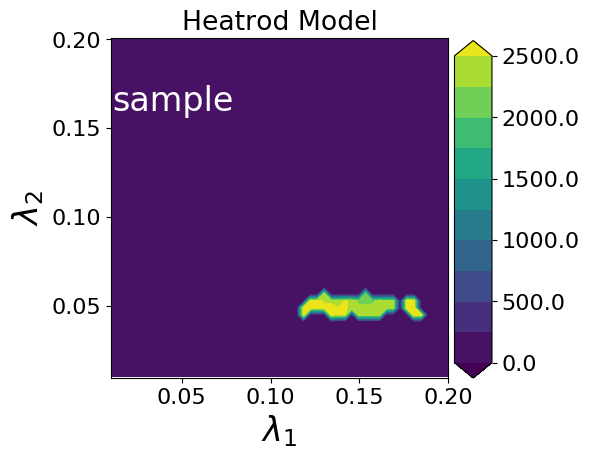
\includegraphics[width=.45\linewidth]{examples/fig_heatrod_q2/HeatrodModel--sample_N500_mc.png}

\caption{The inverse image of the reference measure for $\qoiB$ for $\nsamps = 50$ (top) and $\nsamps = 500$ (bottom). TK - need to remark about how this map may be more precise but it makes it harder to identify the set that contains truth when few model evaluations are available to us (low $\nsamps$). }
\label{fig:heatrod-convergence-b}
\end{figure}


These results motivate further study into utilizing different QoI maps (perhaps some of those other four combinations available to us in this example) depending on where the samples came from in the parameter space.
In general, we saw in this example that given that two maps invert into sets of similar size on average, using the one with lower skewness results in less samples required to accurately approximate the inverse image.
The maps we used had average skewnesses that differed by 0.5 (instead of by 1), and the trend from the linear examples still held in significant portions of the parameter space.

\FloatBarrier

\subsection{Example: Initial Condition and Rate of Something Decaying}\label{ex:decay-set-sample-accuracy}

\begin{figure}[h]
\begin{minipage}{.4\textwidth}
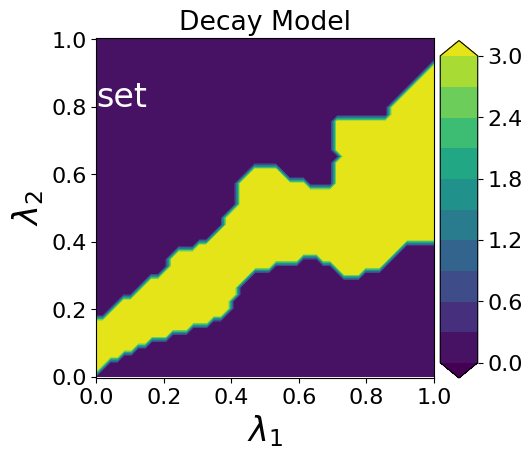
\includegraphics[width=\linewidth]{examples/fig_decay_q1/DecayModel--set_N50_em.png}
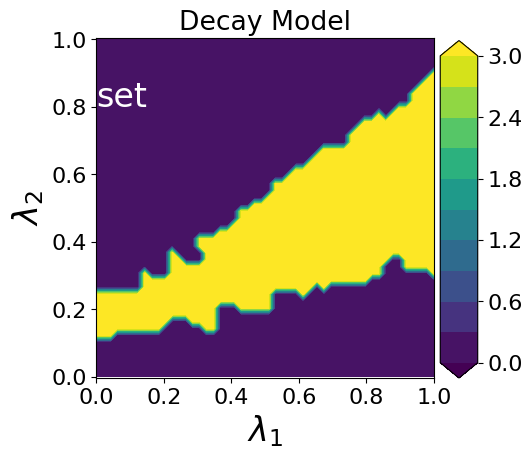
\includegraphics[width=\linewidth]{examples/fig_decay_q1/DecayModel--set_N500_em.png}

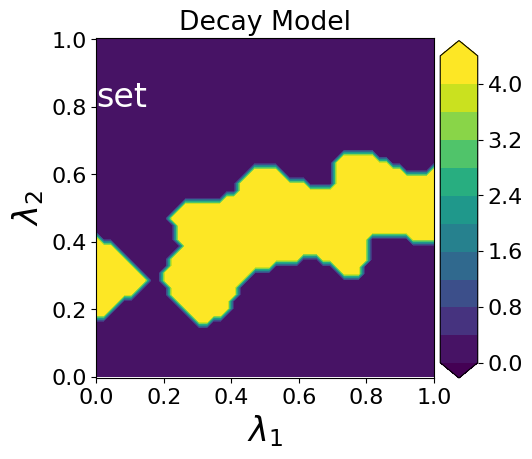
\includegraphics[width=\linewidth]{examples/fig_decay_q2/DecayModel--set_N50_em.png}
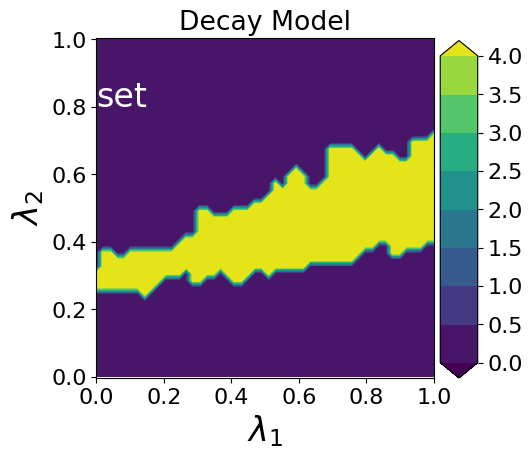
\includegraphics[width=\linewidth]{examples/fig_decay_q2/DecayModel--set_N500_em.png}
\end{minipage}
\begin{minipage}{.4\textwidth}
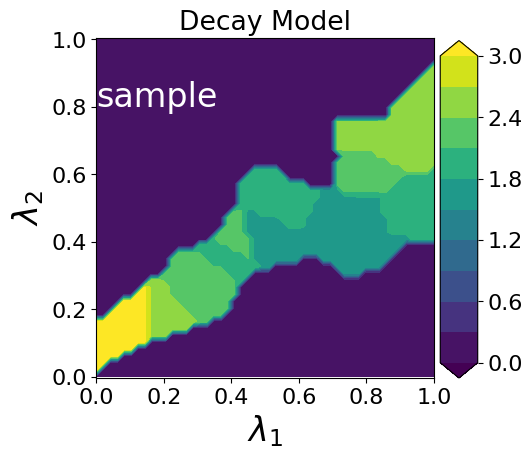
\includegraphics[width=\linewidth]{examples/fig_decay_q1/DecayModel--sample_N50_mc.png}
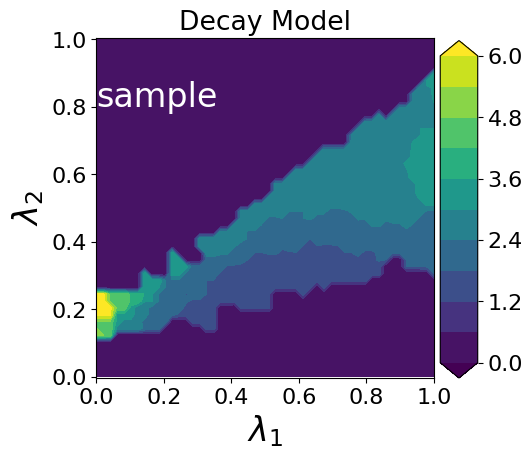
\includegraphics[width=\linewidth]{examples/fig_decay_q1/DecayModel--sample_N500_mc.png}

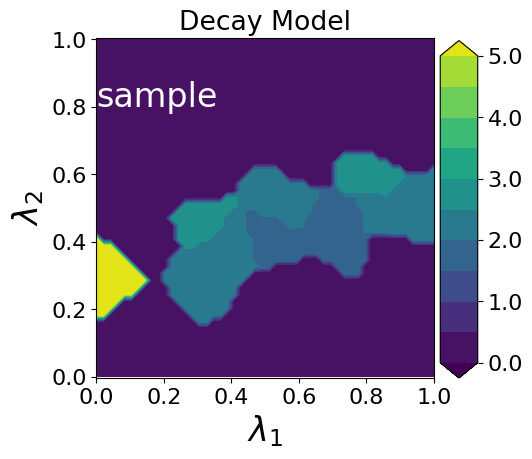
\includegraphics[width=\linewidth]{examples/fig_decay_q2/DecayModel--sample_N50_mc.png}
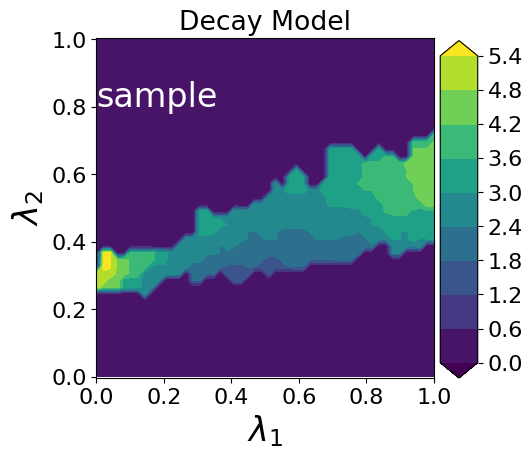
\includegraphics[width=\linewidth]{examples/fig_decay_q2/DecayModel--sample_N500_mc.png}
\end{minipage}

\caption{The inverse image of the reference measure for $\qoiA$ (top half) and $\qoiB$ (bottom half). }
\label{fig:decay-convergence}
\end{figure}

With these nonlinear cases, we find that taking an ``on average'' approach is inefficient, as there can be dramatic differences in the geometric properties of the inverse images in the parameter space depending on the location.
These results motivate further study into utilizing different QoI maps (perhaps some of those other four combinations available to us in this example) depending on where the samples came from in the parameter space.
In general, we saw in this example that given that two maps invert into sets of similar size on average, using the one with lower skewness results in less samples required to accurately approximate the inverse image.
The maps we used had average skewnesses that differed by 0.5 (instead of by 1), and the trend from the linear examples still held in significant portions of the parameter space.

\FloatBarrier
%%%%%%%%%%%%%%
